\section{Results}

In this section we examine the performance of the state-of-the-art RL algorithm PPO for a discrete and continuous action spaces and show how can CL influence the overall learning task. Most of the results for comparison of the discrete action space are taken from our previous paper~\cite{manzl2023relrl}. First subsection presents the results achieved while comparing the trained agent with the same initial parameters using continuous and discrete control schemes. Second subsection describes the work of an agent in a modified environment, where the physical parameters of the system are changed. In the last subsection we present the role of CL in the enhancement of the overall RL agent training. 

\subsection{Reinforcement Learning: discrete vs continuous action space} \label{Reinforcement Learning: discrete vs continuous action space}

To make a comparative analysis we present figures, which illustrate the training performance of an agent via RL-training using in both discrete and continuous action spaces across three different systems: a single-link pendulum (Figure~\ref{fig: training time comparison} (a)), a two-link pendulum (Figure~\ref{fig: training time comparison} (b)), and a three-link pendulum (Figure~\ref{fig: training time comparison} (c)) The discrete action space data, represented by the blue curves, are derived from our previous study of Manzl et. al.~\cite{manzl2023relrl}, while the continuous action space results, represented by the orange curves, are from the current analysis. The vertical dashed lines in each plot indicate the training step at which the agent reaches the maximum number of evaluation tests.
For the single-link system, the agent trained using a continuous action space PPO algorithm achieves optimal performance much faster than the agent trained having the same PPO algorithm but discrete action space. The continuous action space agent stabilizes around 23000 steps, while the discrete agent takes approximately 53,000 steps to achieve a similar level of performance. This indicates that the continuous action space allows for finer control and quicker convergence in simpler systems. The two-link system reveals an even more pronounced difference. The continuous action space agent reaches stable performance at around 46000 steps, significantly ahead of the discrete action space agent, which stabilizes much later at around 101,000 steps. The continuous agent not only converges faster but also exhibits higher stability in maintaining optimal rewards throughout training. In the more complex three-link system, the advantage of the continuous action space is evident once again. The continuous agent reaches optimal performance at around 270000 steps, whereas the discrete agent takes over 500,000 steps to achieve comparable results. Notably, the discrete agent experiences significant fluctuations in performance, underscoring the challenges posed by the increased complexity when using a discrete action space.

\begin{figure}[h!]
	\centering
	\begin{subfigure}[t]{0.48\textwidth}
		\centering
		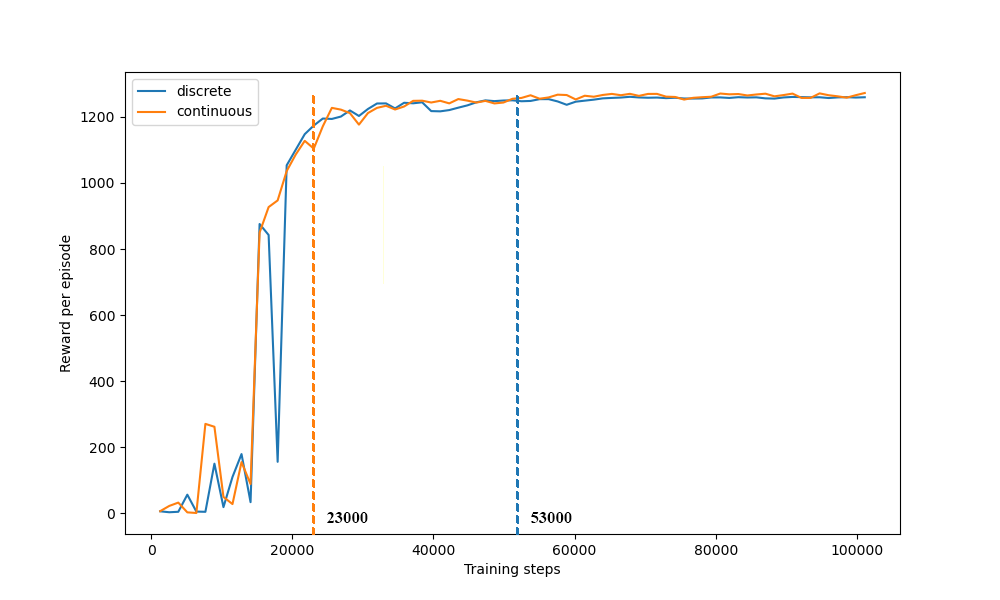
\includegraphics[width=\textwidth]{Figures/SP_discrete_vs_continuous_training_time.png}
		\label{fig: sp - training time}
		\caption{1-link system. Agent in continuous action space reaches maximum number of successful tests in approximately of 23000 timesteps.}
	\end{subfigure}
	\hfill
	\begin{subfigure}[t]{0.48\textwidth}
		\centering
		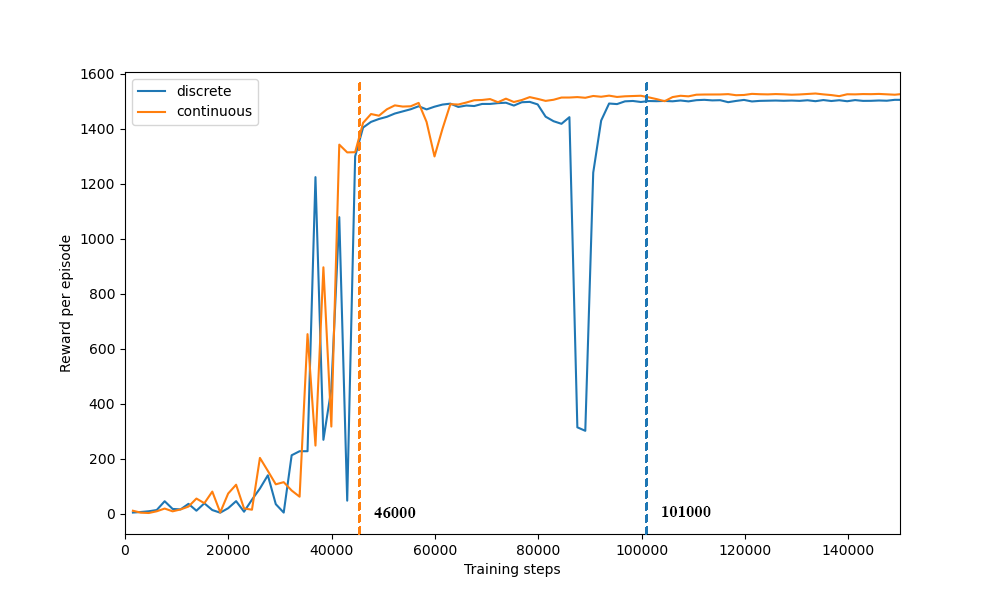
\includegraphics[width=\textwidth]{Figures/DP_discrete_vs_continuous_training_time.png}
		\label{fig: dp - training time}
		\caption{2-link system. At the timesteps of 46000 the agent has reached the maximum number of successful tests.}
	\end{subfigure}
	\begin{subfigure}[t]{0.48\textwidth}
		\centering
		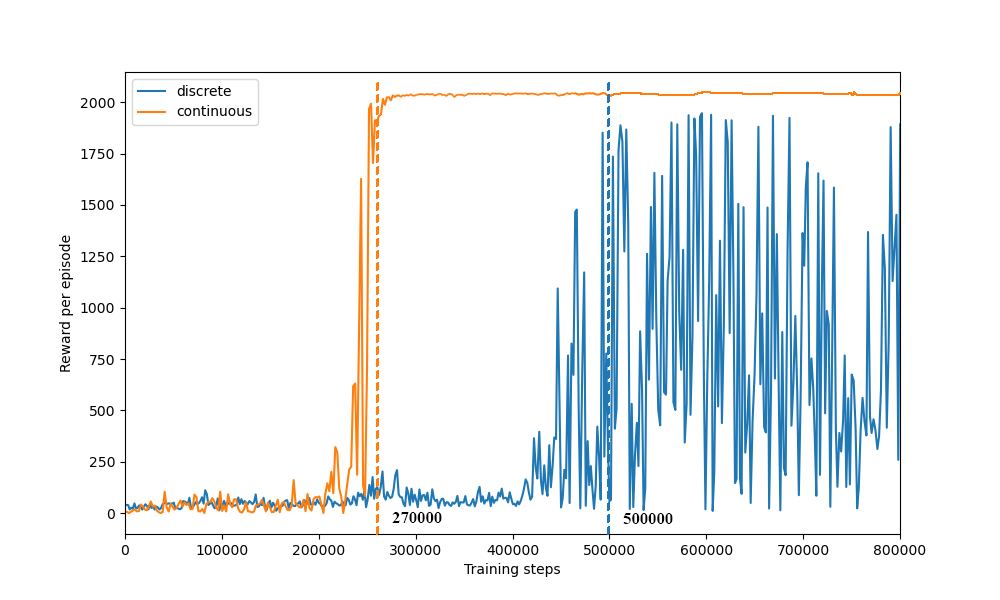
\includegraphics[width=\textwidth]{Figures/TP_discrete_vs_continuous_training_time.png}
		\label{fig: tp - training time}
		\caption{3-link system. Less then 300000 timesteps required to train the system with the usage of continuous action space.}
	\end{subfigure}
	
	\caption{Training times for the PPO agents for 1-link (a), 2-link (b) and 3-link (c) systems}
	\label{fig: training time comparison}
\end{figure}

The continuous action space consistently demonstrates superior stability across all systems, as reflected in the smoother reward curves after convergence. It also reduces training time on up to 50\% for an agent to achieve a maximum number of successful tests. In contrast, the discrete action space leads to more oscillatory performance, particularly in more complex systems, which could indicate less efficient exploration and exploitation during training.

For a deeper evaluation of the continuous control scheme in comparison to the discrete one, we have created a stability zone, the development of which is described in our work of Manzl et al.~\cite{manzl2023relrl}. From an engineering standpoint, not only are the randomized tests used for evaluation important, but it is also crucial to identify an area where the agent successfully performs the stabilization task for practical, real-world applications. The stability zones are shown in Figure~\ref{fig: continuous vs discrete} and illustrate the performance of discrete (orange) and continuous (light yellow) action spaces. These zones represent the regions in state space where the agent successfully maintains the pendulum's stability. The axes represent different state variables depending on the system's complexity, as detailed below.
For the 1-link system (Figure~\ref{fig: continuous vs discrete} (a)) the stability zones are depicted as elongated regions around the origin where the pendulum is successfully balanced. X-axis represent the link's angle and Y-axis its angular velocity. The continuous action space encompasses a slightly broader area compared to the discrete action space, indicating a greater tolerance for variations in the angle and angular velocity. This suggests that the continuous action space provides more flexibility in controlling the pendulum, allowing it to stabilize from a wider range of initial conditions. For the 2-link system (Figure~\ref{fig: continuous vs discrete} (b)), the stability zones are narrower and more elongated, reflecting the increased complexity of the system. First and the second link angle combinations are presented in this zone. The continuous action space again covers a slightly larger area than the discrete action space, particularly along the axis. This expanded zone suggests that the continuous action space better handles the interactions between the two links, allowing for more robust stabilization strategies. In the 3-link system (Figure~\ref{fig: continuous vs discrete} (c) and Figure~\ref{fig: continuous vs discrete} (d)), the stability zones become even more restricted, particularly in the second plot, where the angles of the second and third links are plotted. The continuous action space consistently outperforms the discrete space by maintaining a larger stability region in both plots. The narrower orange zones indicate that the discrete action space struggles with the additional degrees of freedom, whereas the continuous action space adapts more effectively to the system's increased complexity.

\begin{figure}[h!]
	\centering
	\begin{subfigure}[t]{0.48\textwidth}
		\centering
		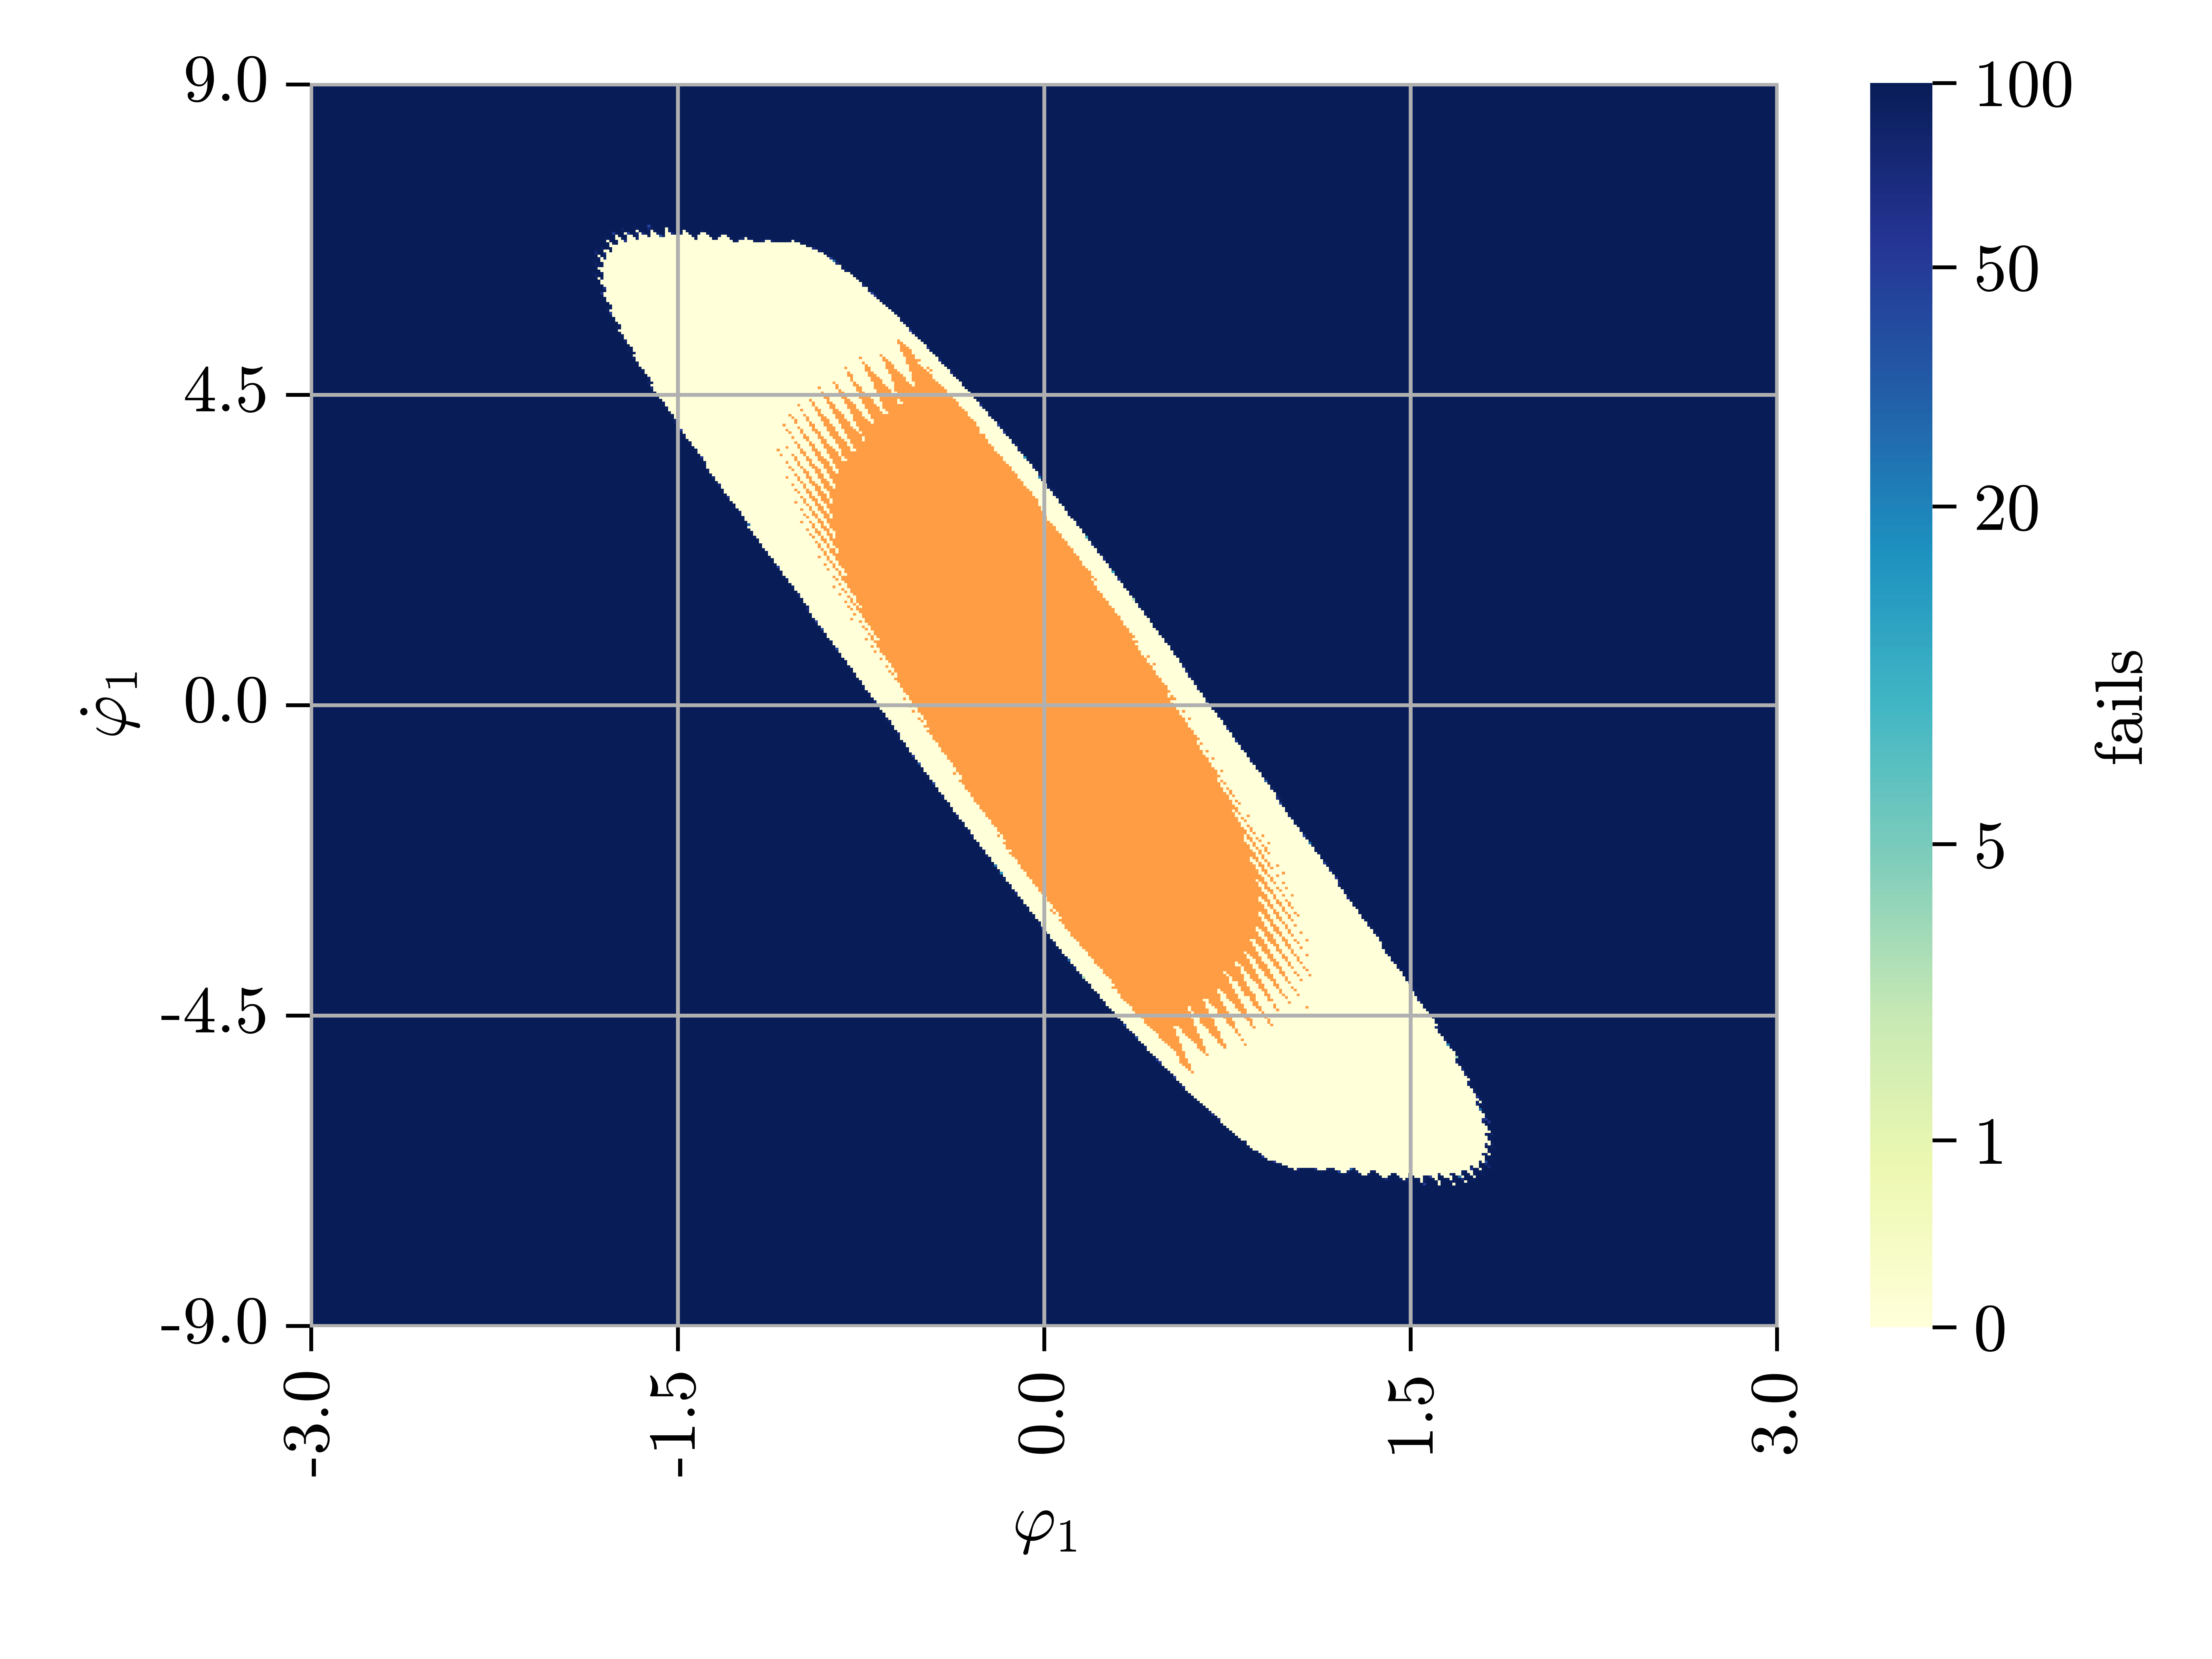
\includegraphics[width=\textwidth]{Figures/SP_continuous_vs_discrete_phi1phi1dot.png}
		\label{fig: sp - continuous vs discrete}
		\caption{}
	\end{subfigure}
	\hfill
	\begin{subfigure}[t]{0.48\textwidth}
		\centering
		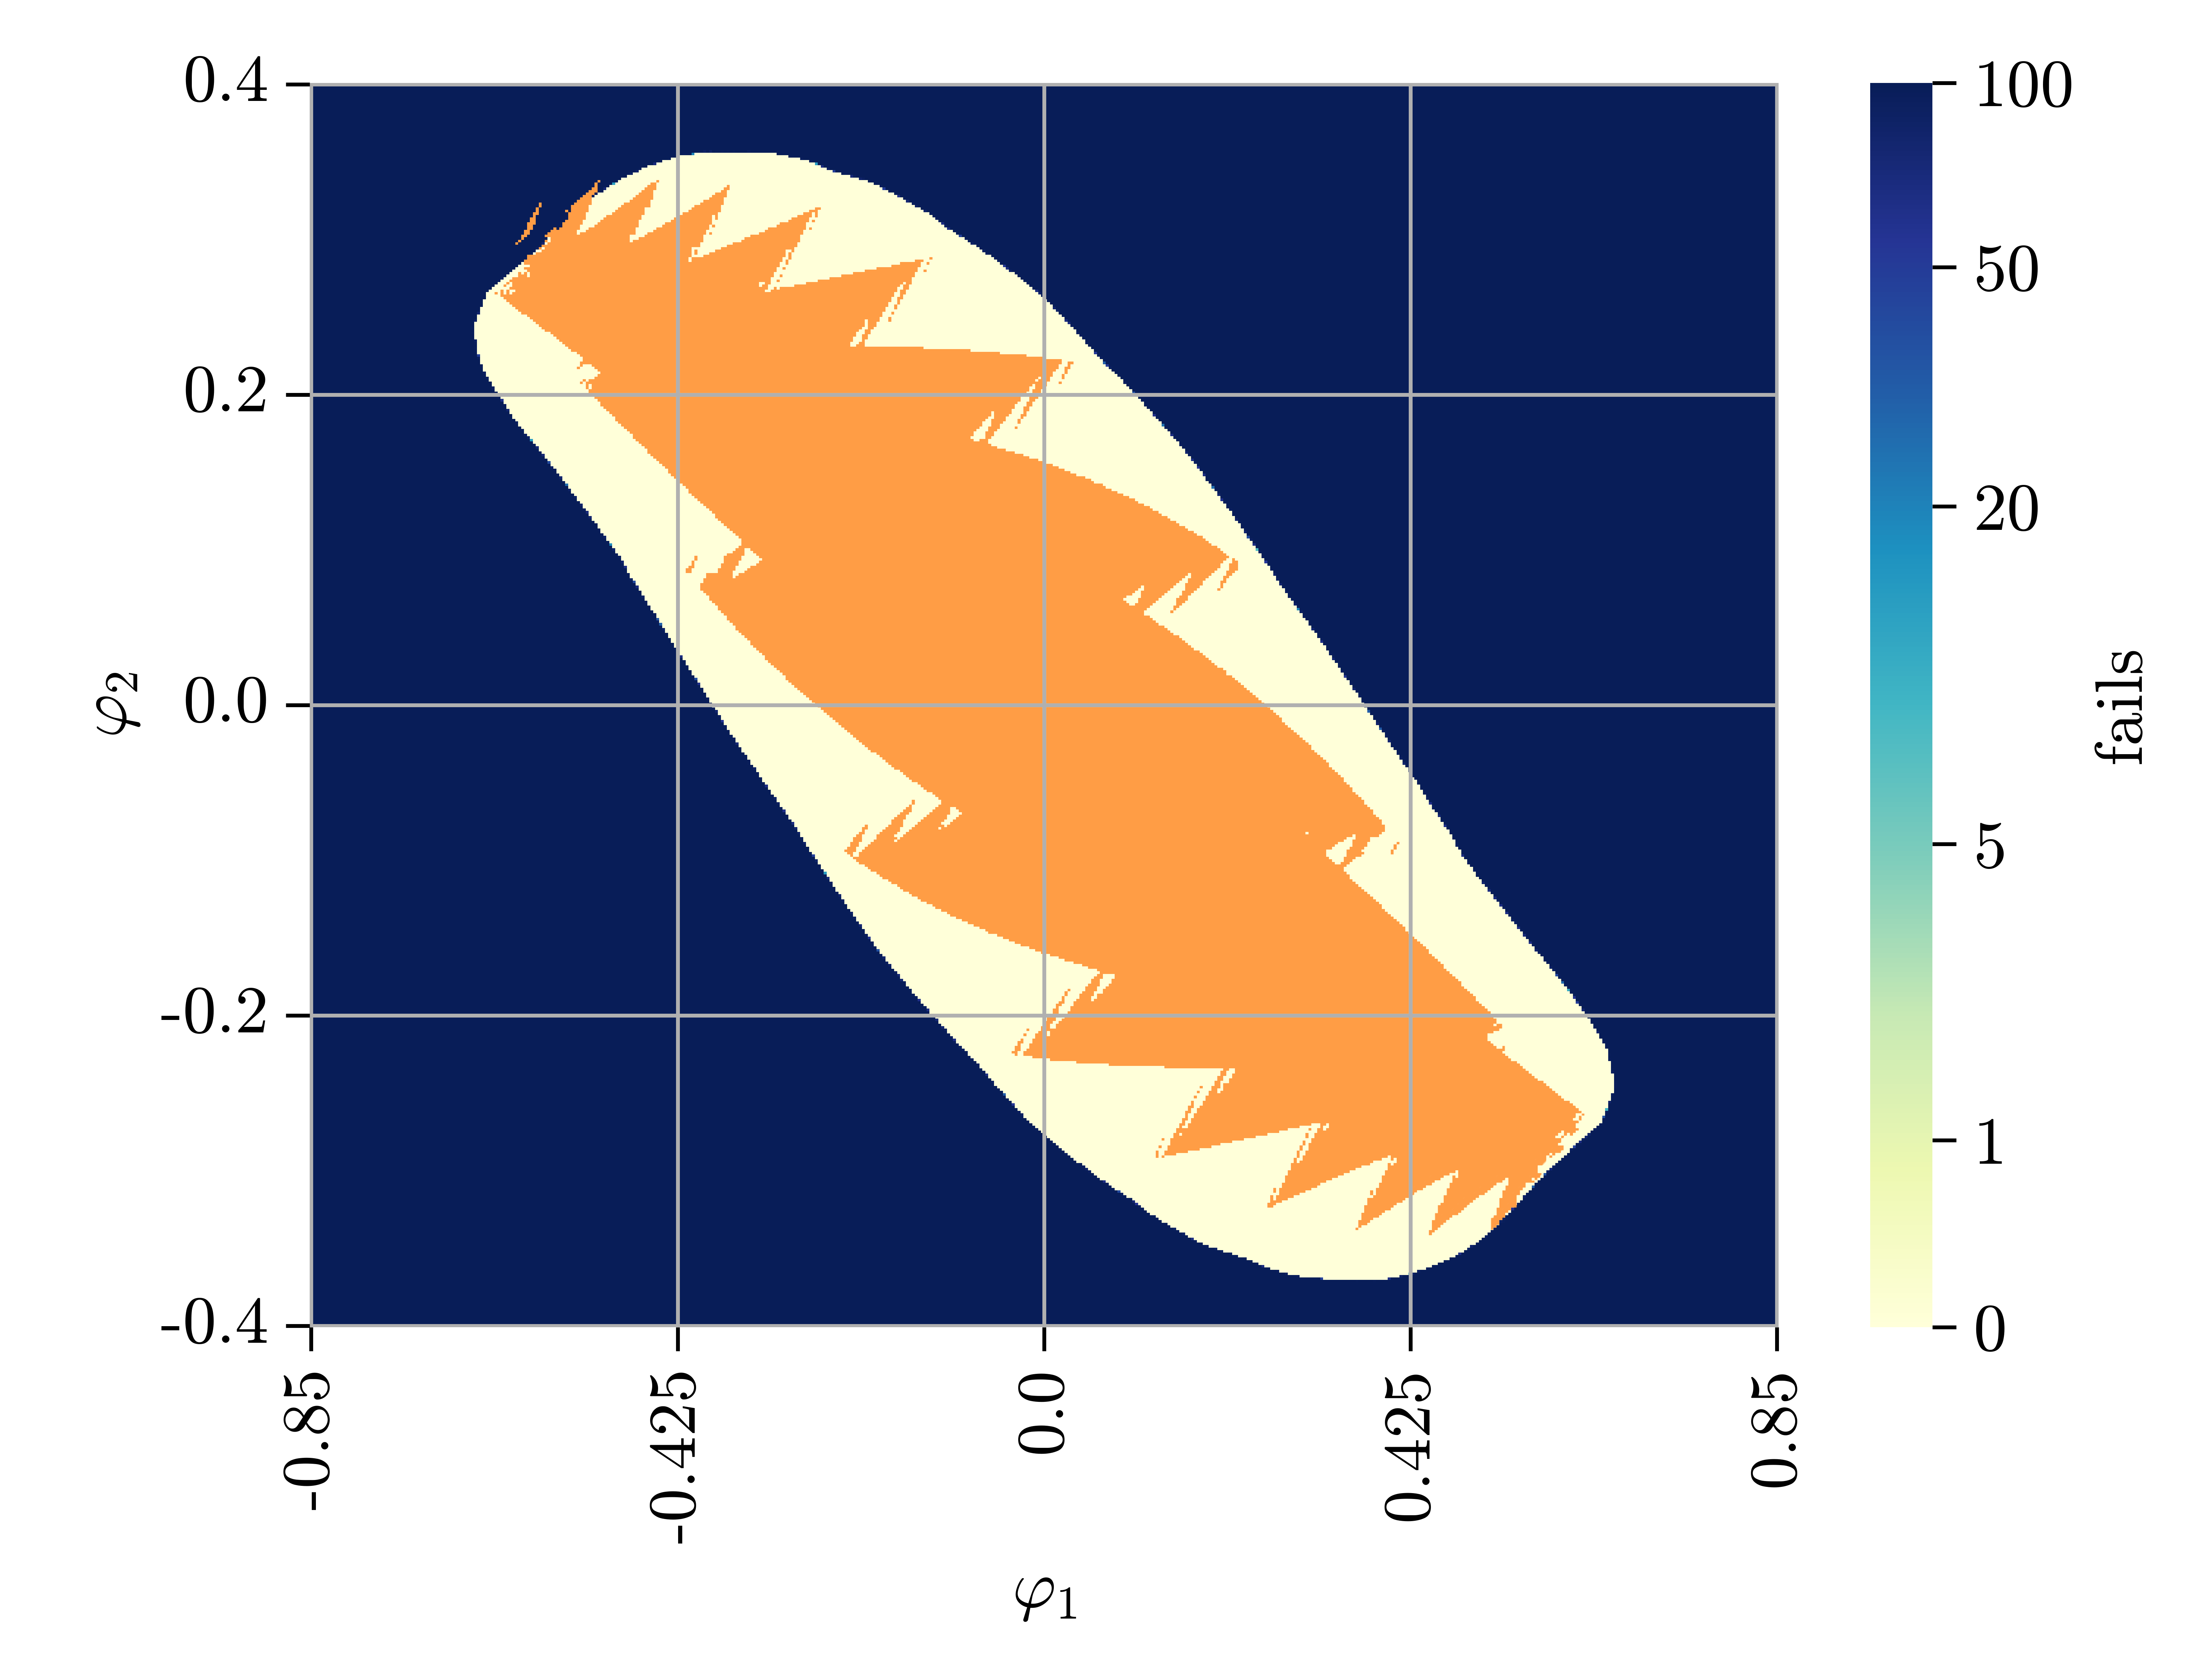
\includegraphics[width=\textwidth]{Figures/DP_continuous_vs_discrete_phi1phi2.png}
		\label{fig: dp - continuous vs discrete}
		\caption{}
	\end{subfigure}
	
	\vspace{0.2cm}
	
	\begin{subfigure}[t]{0.48\textwidth}
		\centering
		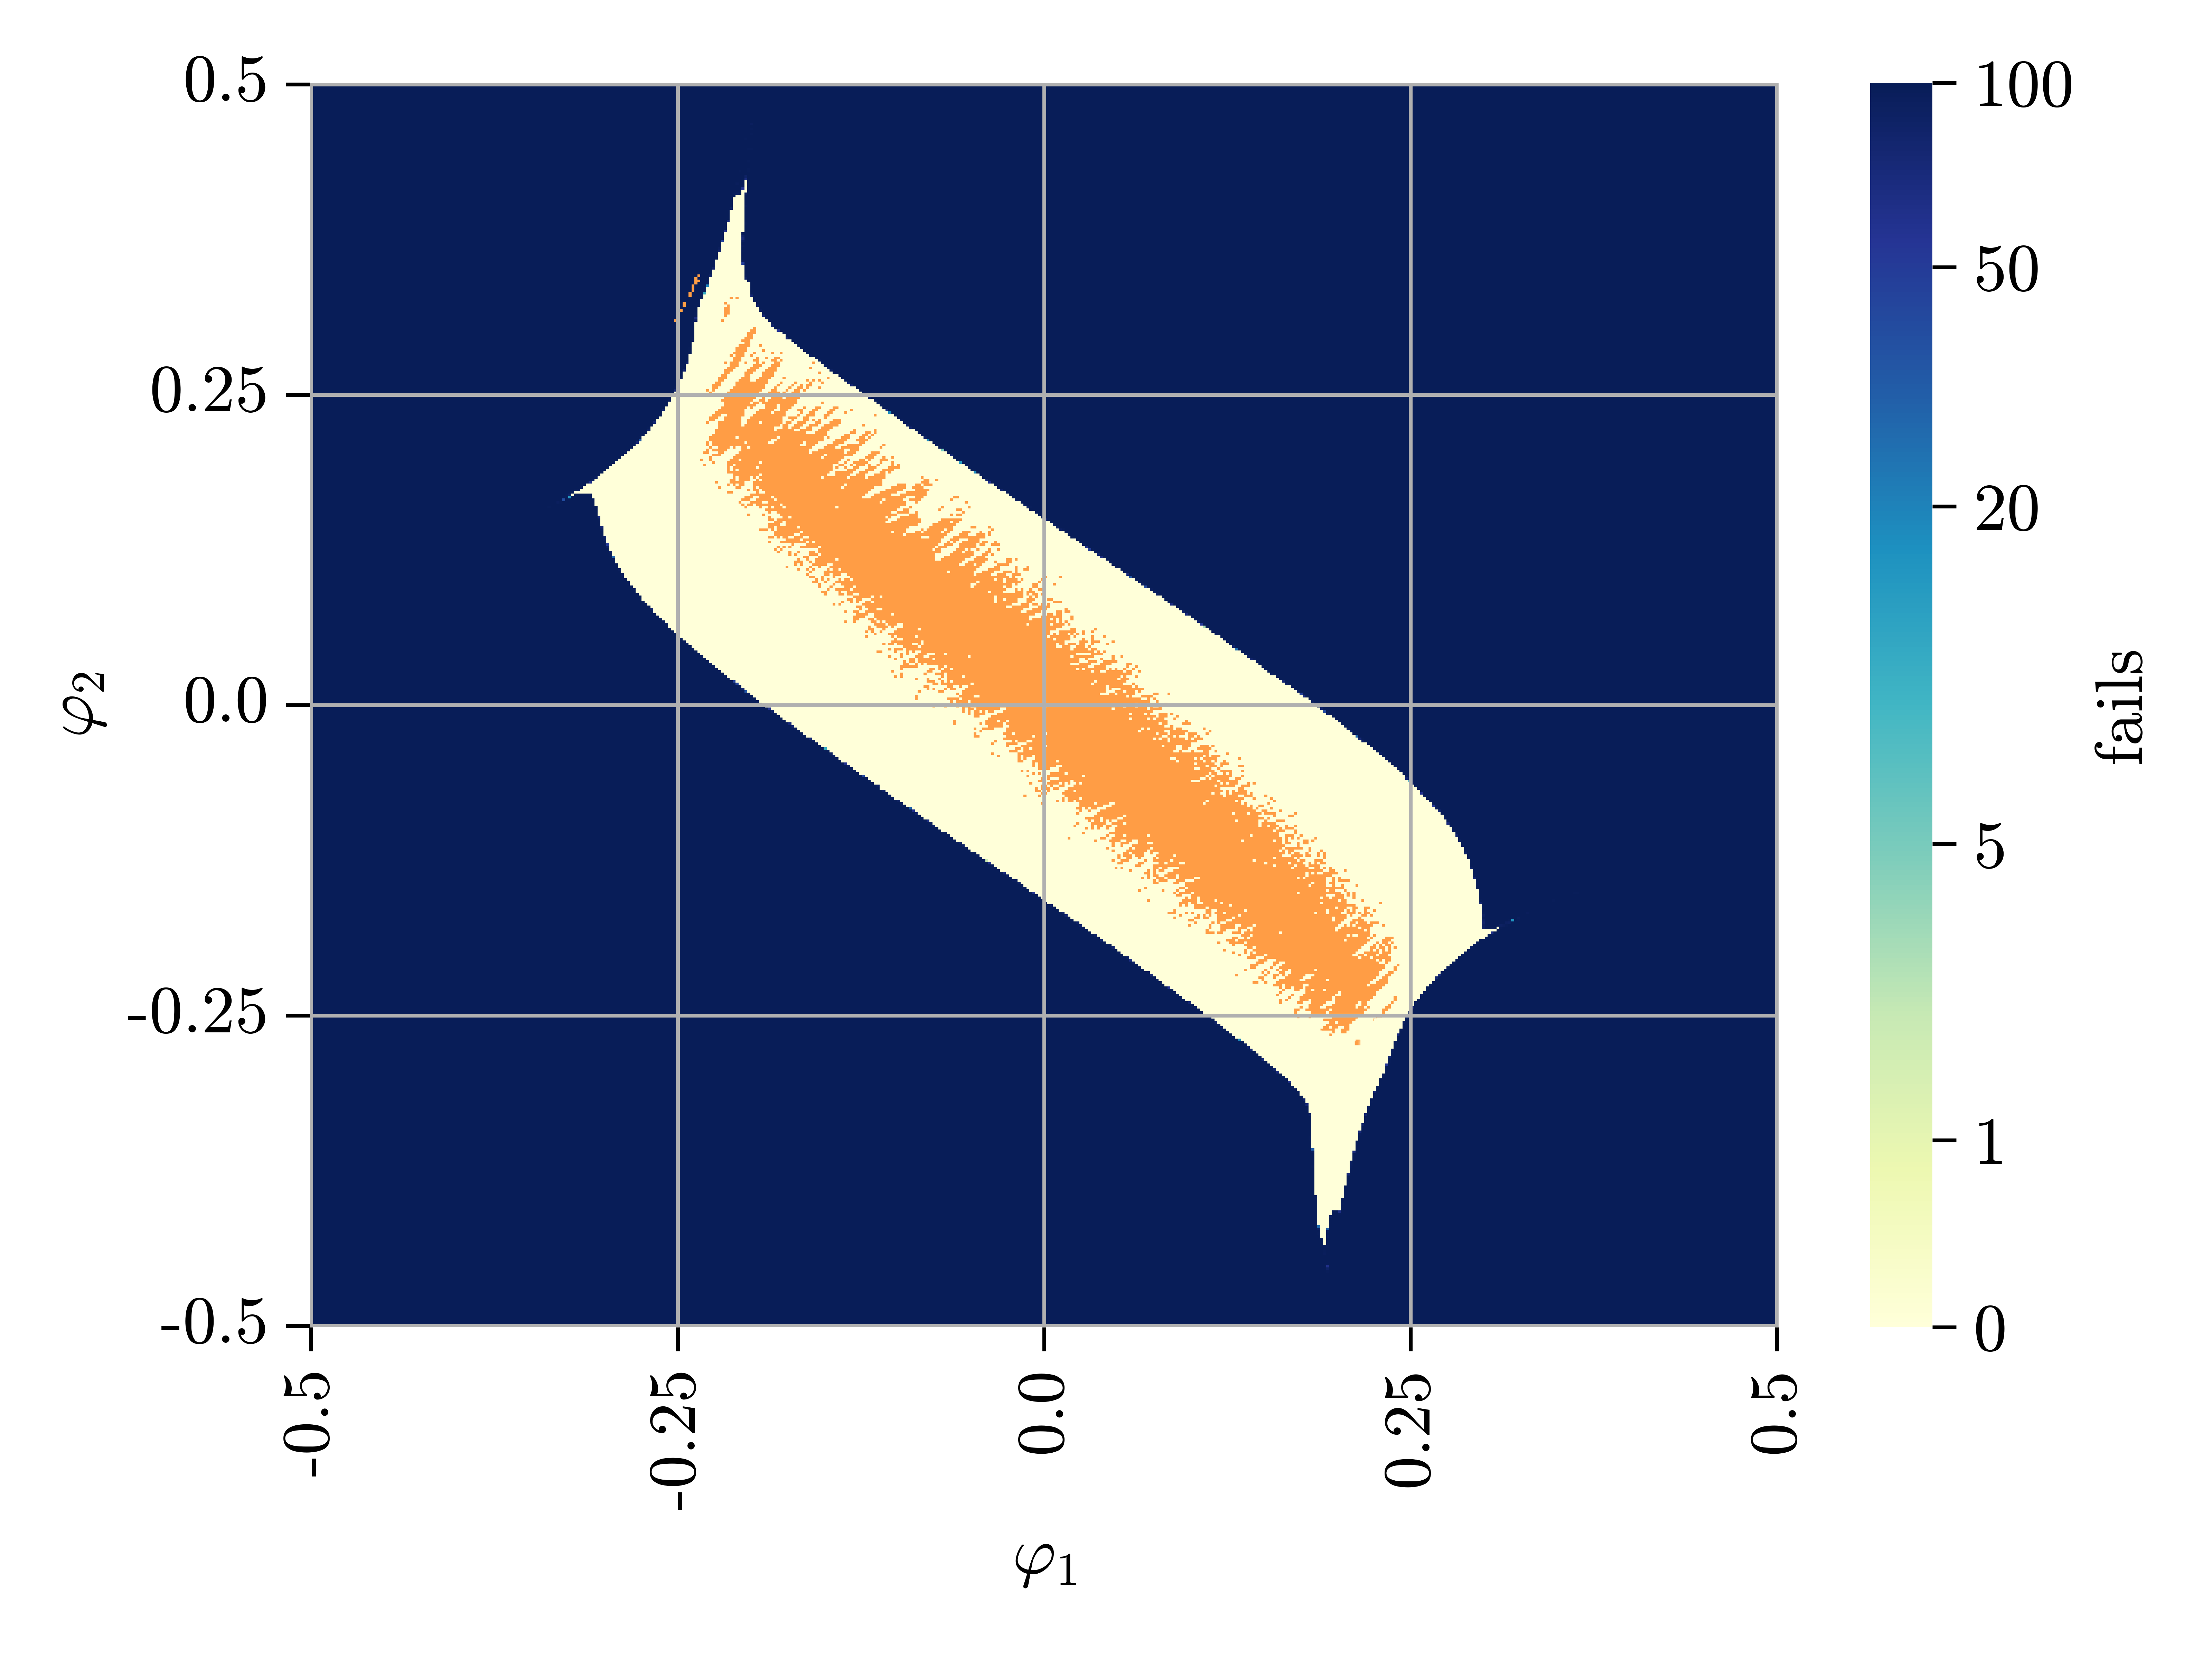
\includegraphics[width=\textwidth]{Figures/TP_continuous_vs_discrete_phi1phi2.png}
		\label{fig: tp - continuous vs discrete, phi1 phi2}
		\caption{}
	\end{subfigure}
	\hfill
	\begin{subfigure}[t]{0.48\textwidth}
		\centering
		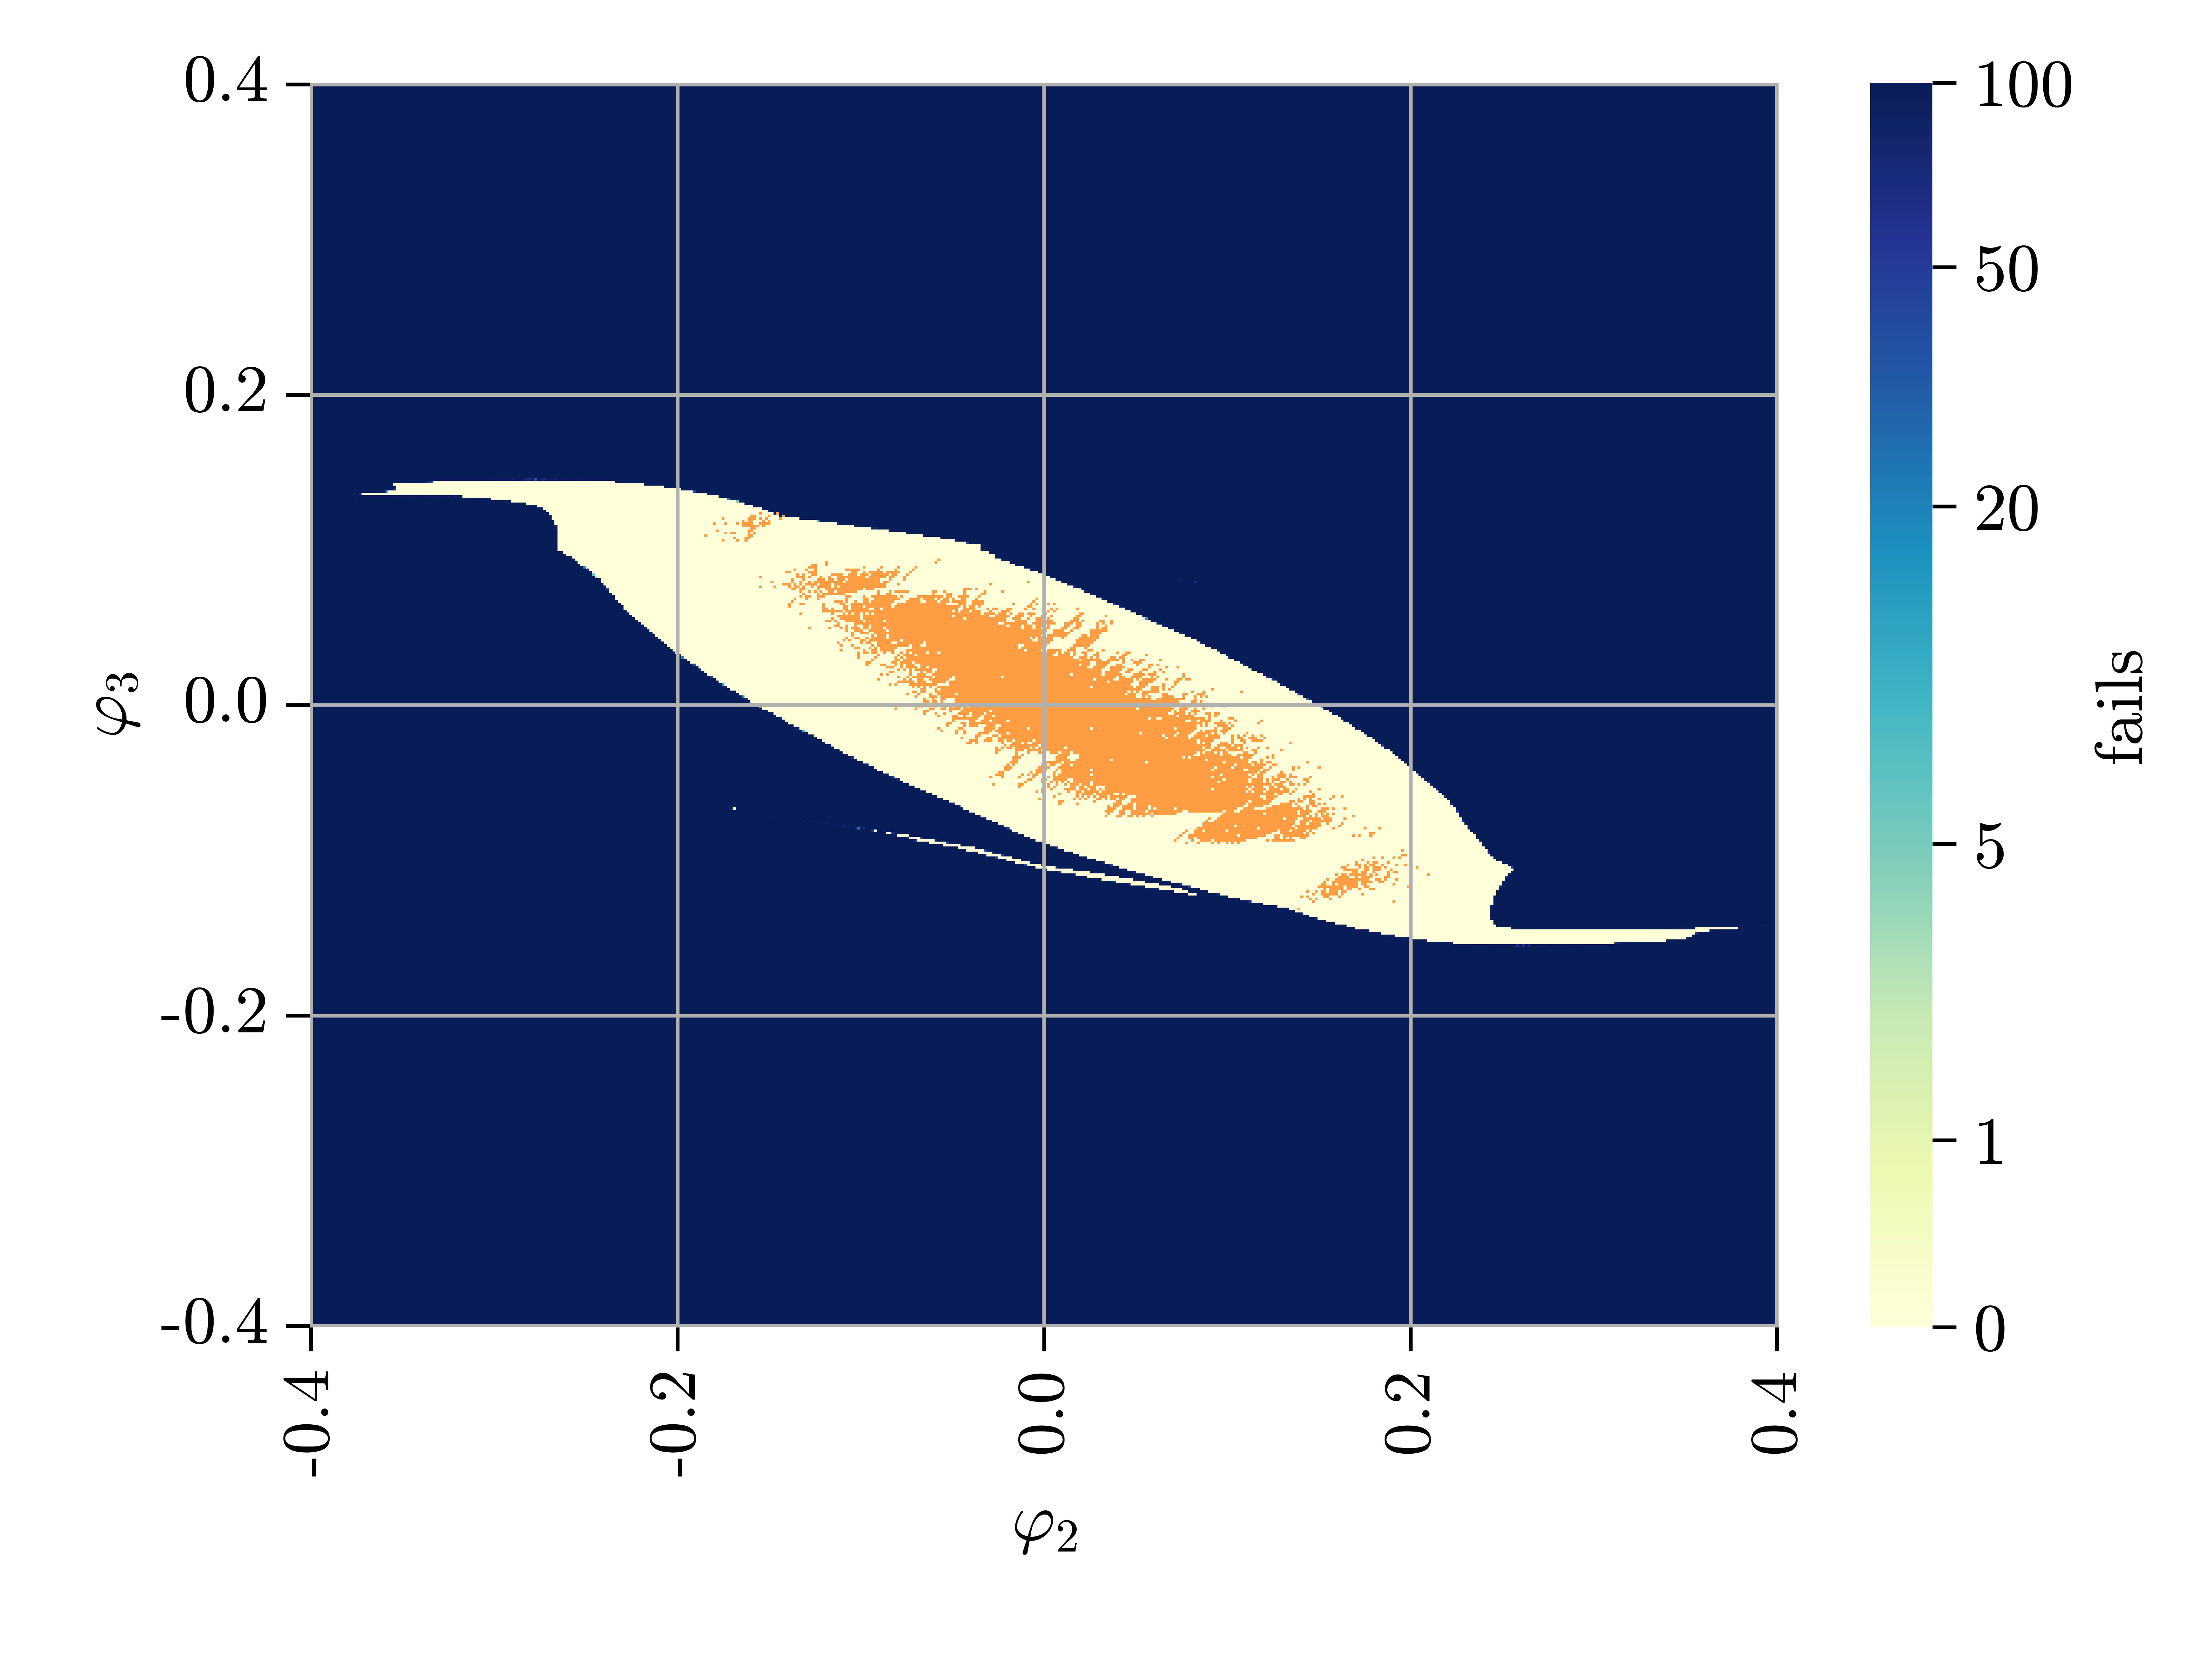
\includegraphics[width=\textwidth]{Figures/TP_continuous_vs_discrete_phi2phi3.png}
		\label{fig: tp - continuous vs discrete, phi2 phi3}
		\caption{}
	\end{subfigure}
	
	\caption{Stability zones comparison of the PPO agent using different control strategies. For the 1-link system (a) the zone axis are link's angle $\phi_1$ and angular velocity $\dot{\phi_1}$, while for the 2-link system (b) axis are the pendulum link angles $\phi_1$ and $\phi_2$. Figures (b) and (c) present the stability zones based on the dependence of pendulum link angles of $\phi_1$ and $\phi_2$ and of $\phi_2$ and $\phi_3$. The discrete control stability zone is indicated in orange; continuous is in white beige. Each grid cell represents 100 randomized tests.}
	\label{fig: continuous vs discrete}
\end{figure}

These stability zones highlight the advantages of continuous action spaces in maintaining the stability of multi-link inverted pendulum systems. As the system's complexity increases (from 1-link to 3-link), the continuous action space's broader stability regions suggest a higher robustness to variations in state variables, making it more effective in stabilizing complex systems.
The continuous action space's ability to control a wider range of initial conditions is particularly beneficial in systems with multiple degrees of freedom, where precise and adaptive control strategies are required. This is evident in the progressively more complex systems, where the continuous action space maintains larger stability zones, indicating better overall performance.
These findings support the notion that continuous action spaces may be more suitable for applications requiring fine-tuned control in high-dimensional environments, where the ability to handle a broader range of state variations is crucial for success.

\subsection{Agents with continuous action space tested on modified environments} \label{subsec: Agent tested on modified environments}

In this section, we examine the impact of changing properties of the environment, namely
link length, mass, and added friction, on the stability zones. The friction is implemented in the same fashion as in our previous study~\cite{manzl2023relrl} and is modeled using Coulomb friction, characterized by a friction torque, which opposes rotation and is independent of the applied forces. The investigation is conducted
using the inverted double pendulum on a cart model (same continuous agent as in the Figure~\ref{fig: continuous vs discrete} (b)). In each subplot of Figure~\ref{fig: agent impact on different environments}, the stability zone is determined for the same agent in various modified environments, and the contour of the stability zone from the original environment is overlaid.

 \begin{figure}[h!]
     \centering
     \begin{subfigure}[t]{0.32\textwidth}
         \centering
         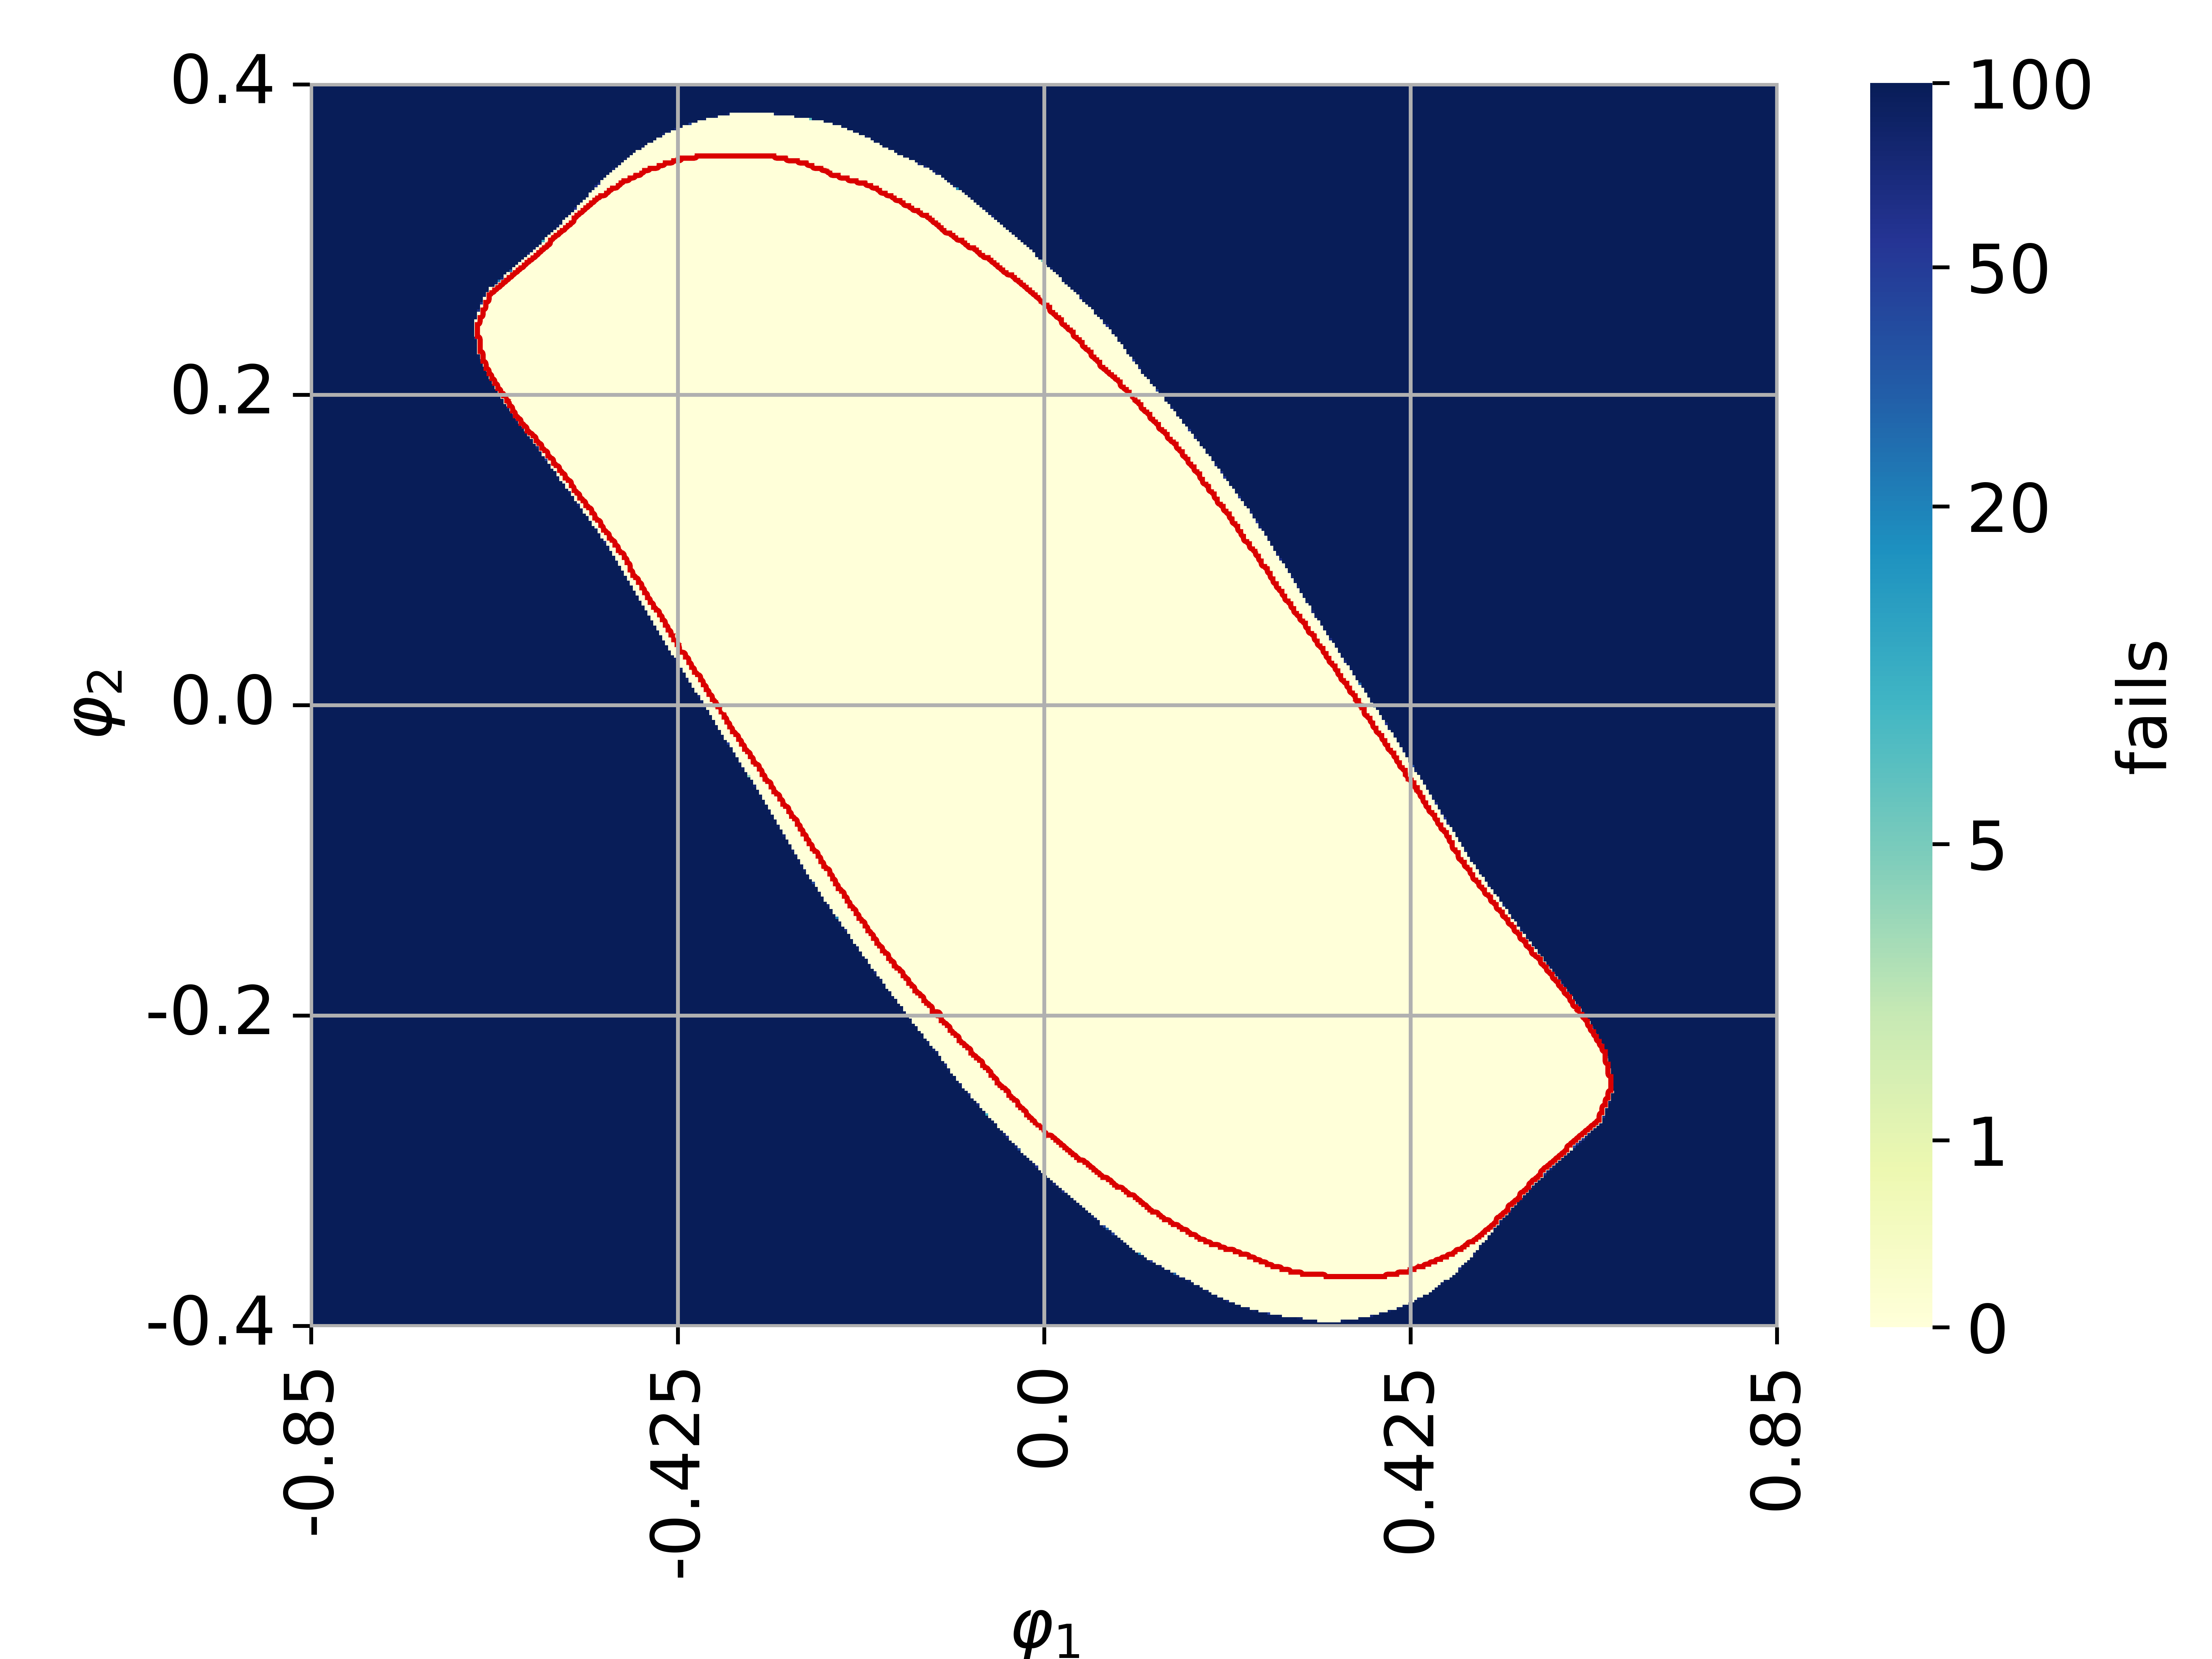
\includegraphics[width=\textwidth]{Figures/DP_len_1.1.png}
         \label{fig: DP len 1.1}
         \caption{}
     \end{subfigure}
     \hfill
     \begin{subfigure}[t]{0.32\textwidth}
         \centering
         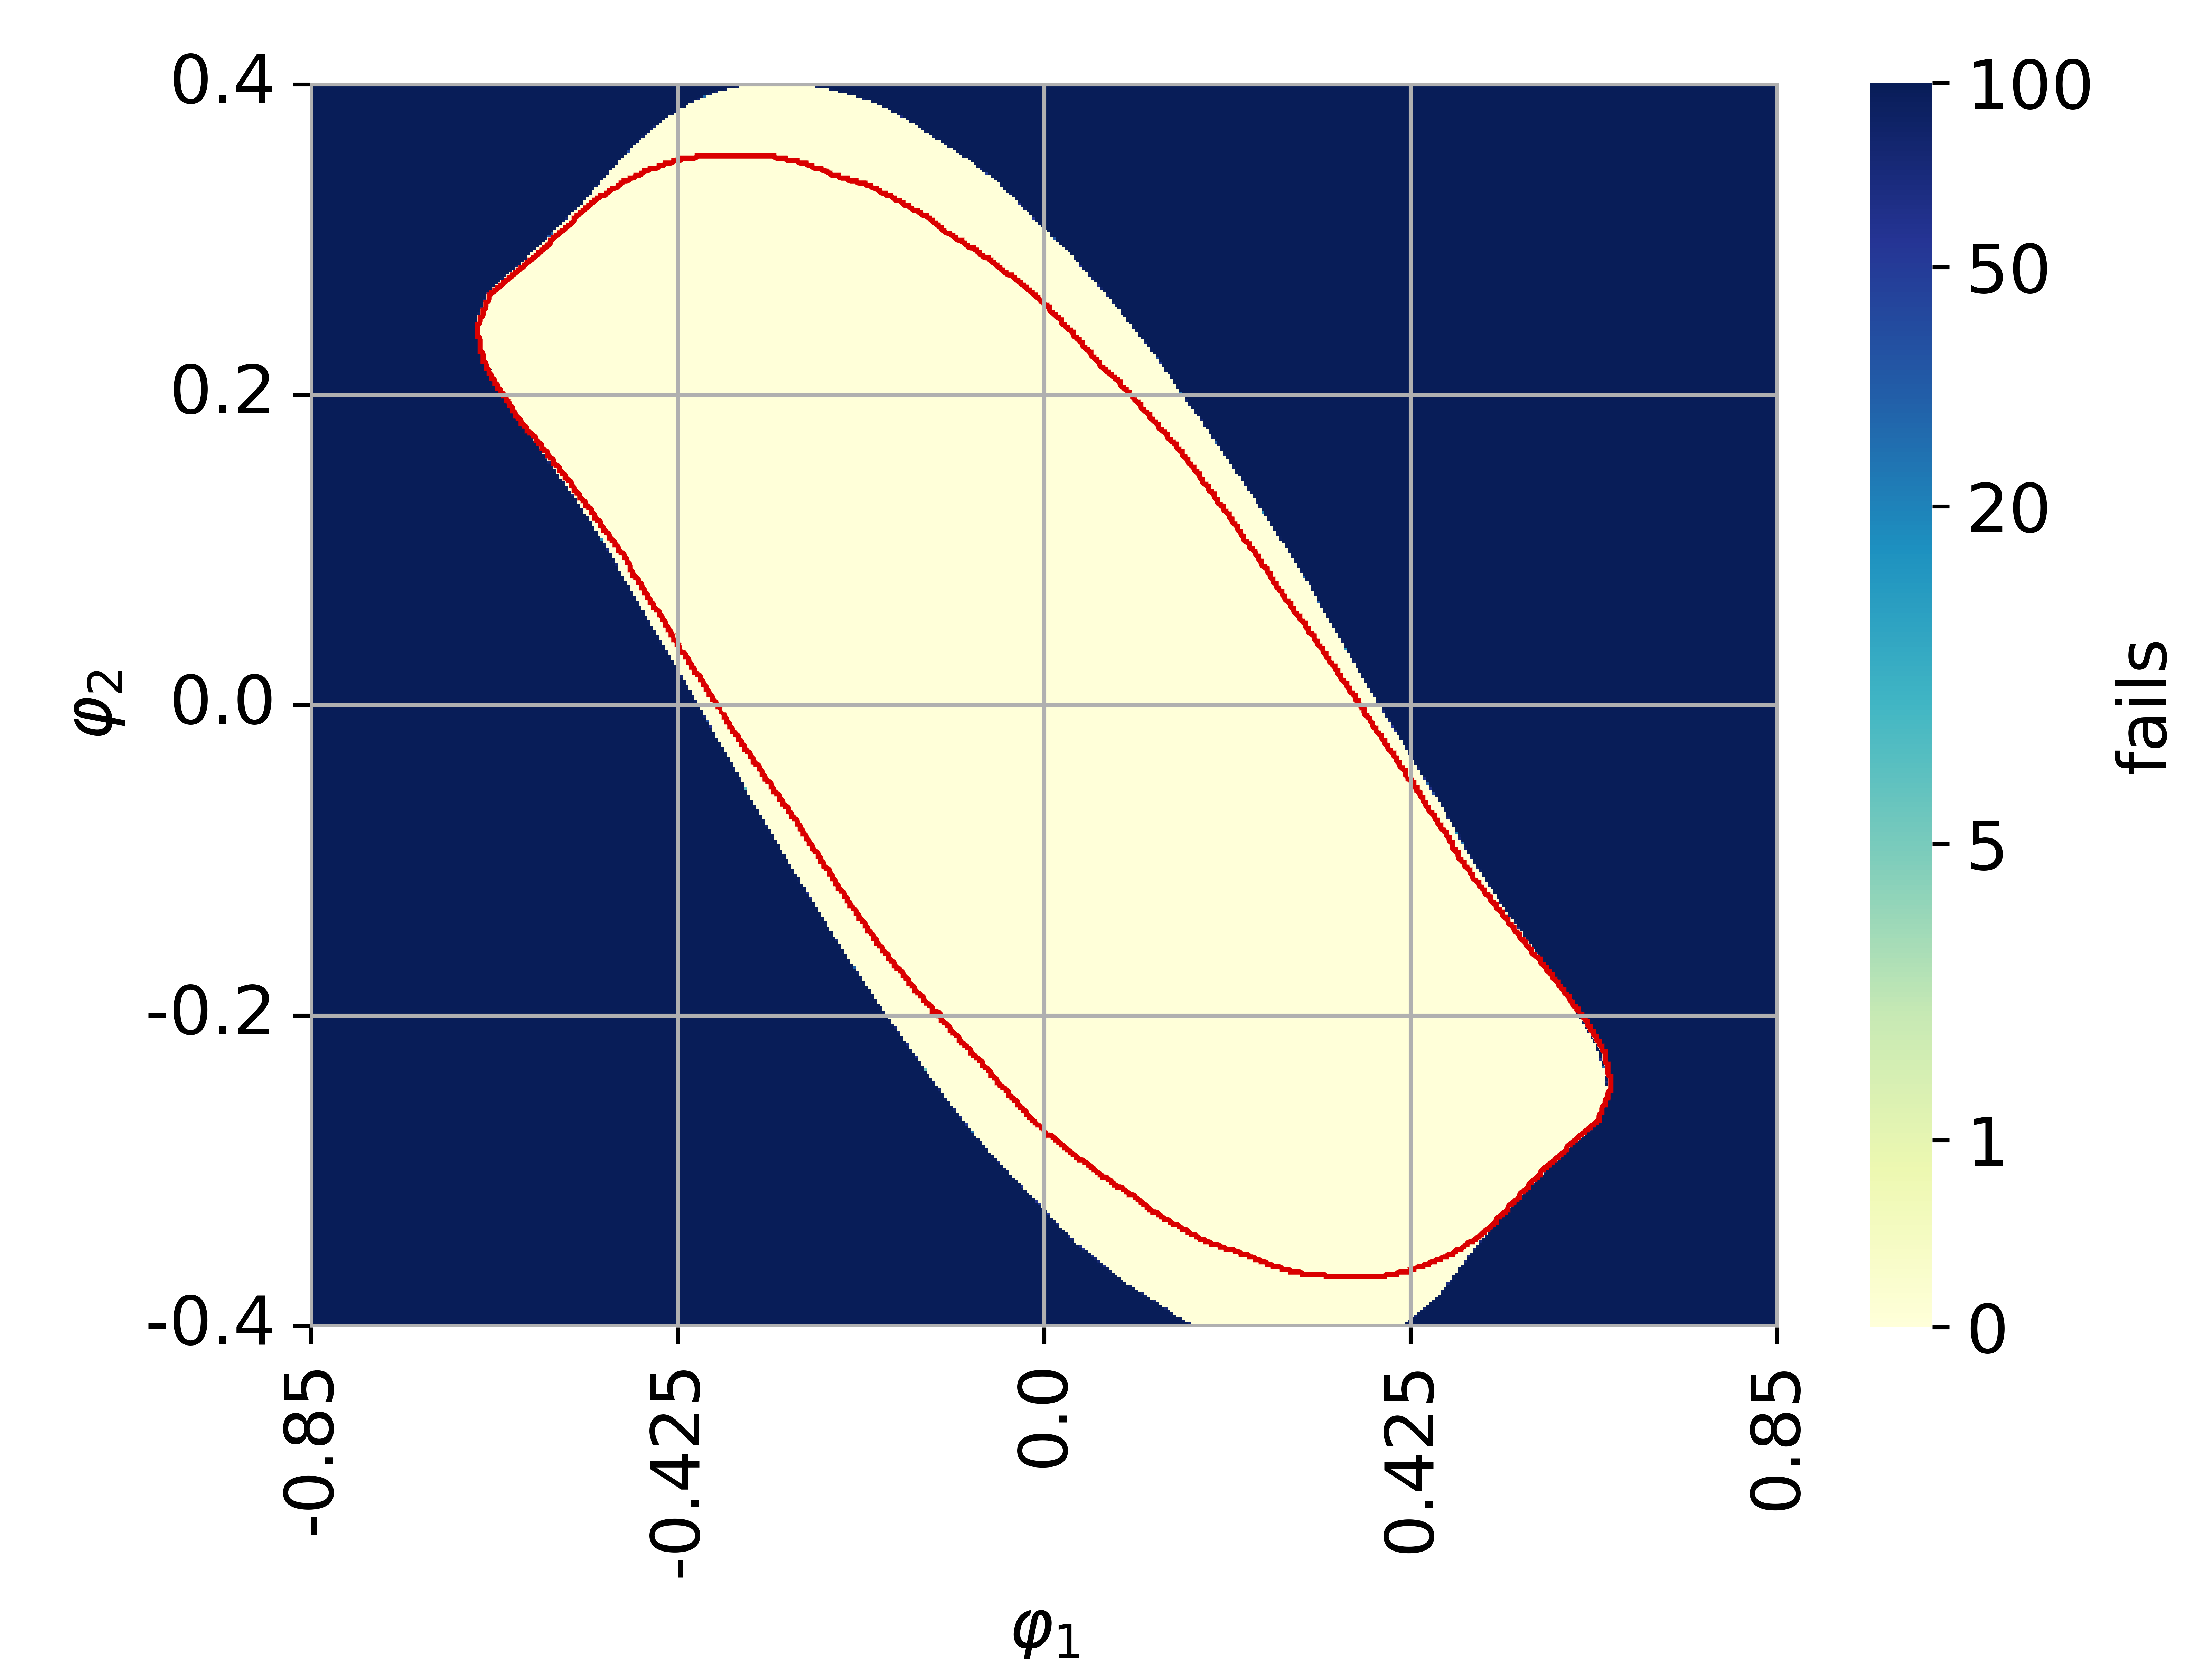
\includegraphics[width=\textwidth]{Figures/DP_len_1.2.png}
         \label{fig: DP len 1.2}
         \caption{}
     \end{subfigure}
     \hfill
     \begin{subfigure}[t]{0.32\textwidth}
         \centering
         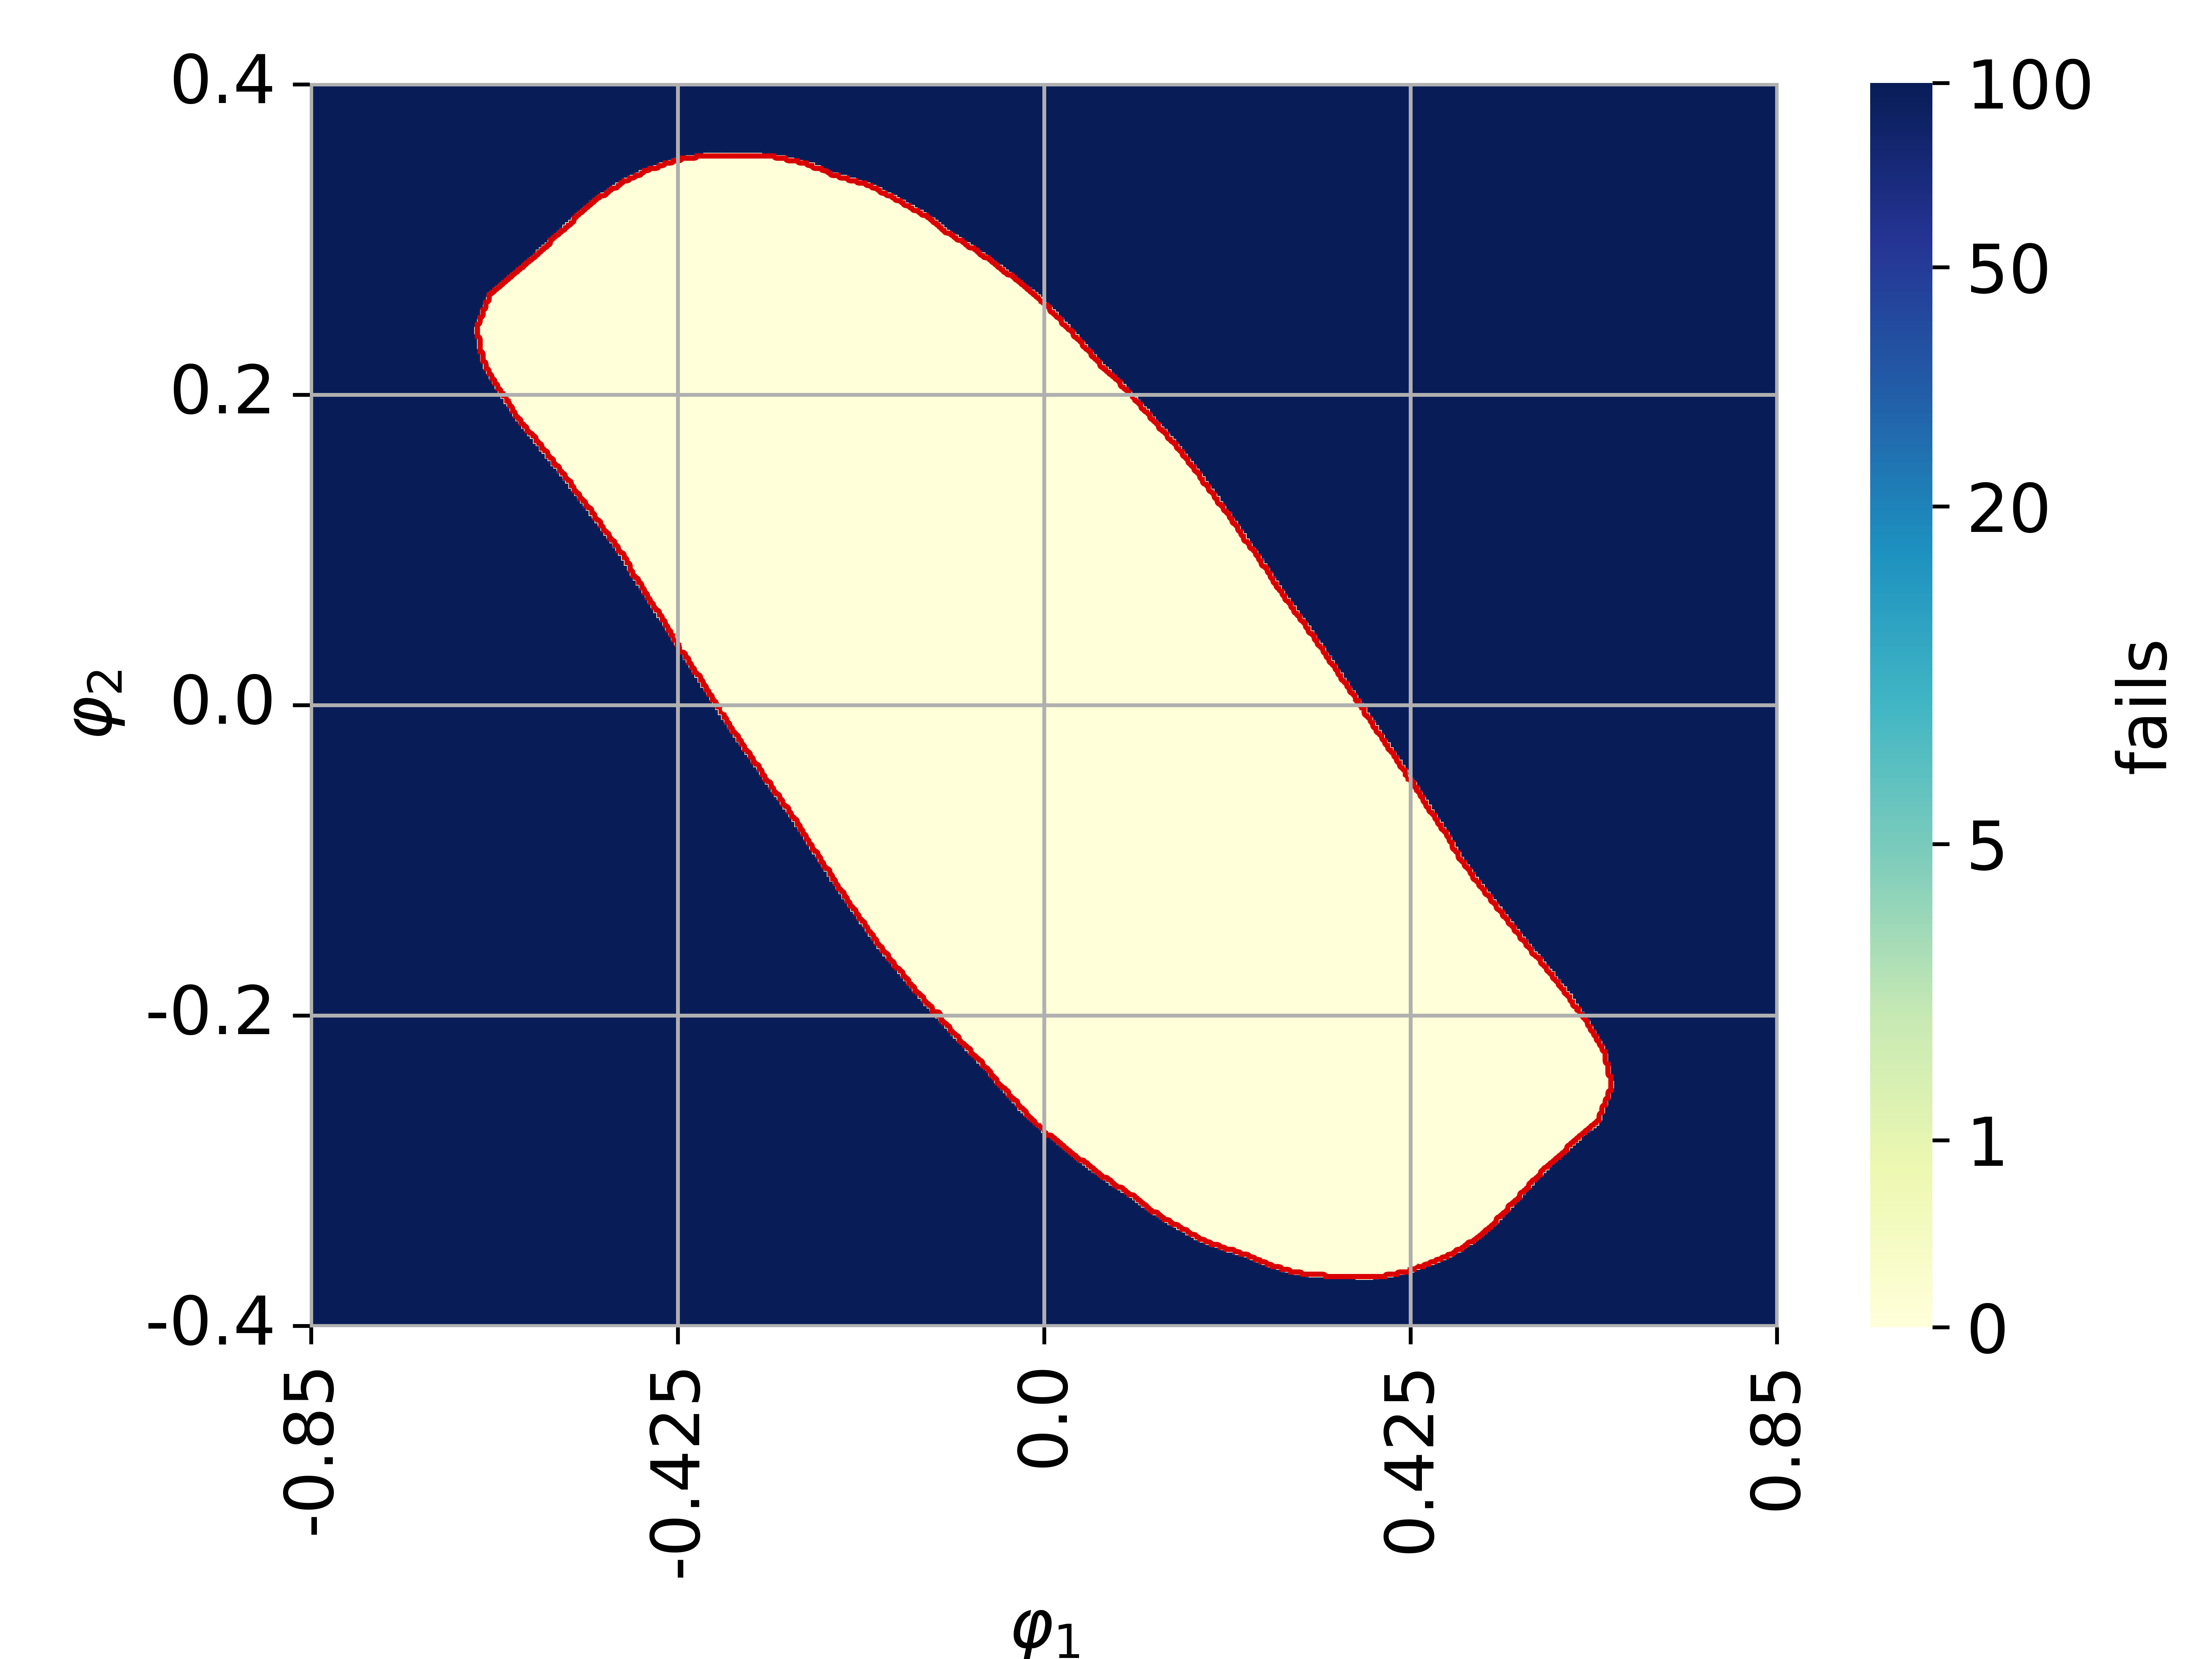
\includegraphics[width=\textwidth]{Figures/DP_mass_1.1.png}
         \label{fig: DP mass 1.1}
         \caption{}
     \end{subfigure}

     \vspace{0.2cm}

     \begin{subfigure}[t]{0.32\textwidth}
         \centering
         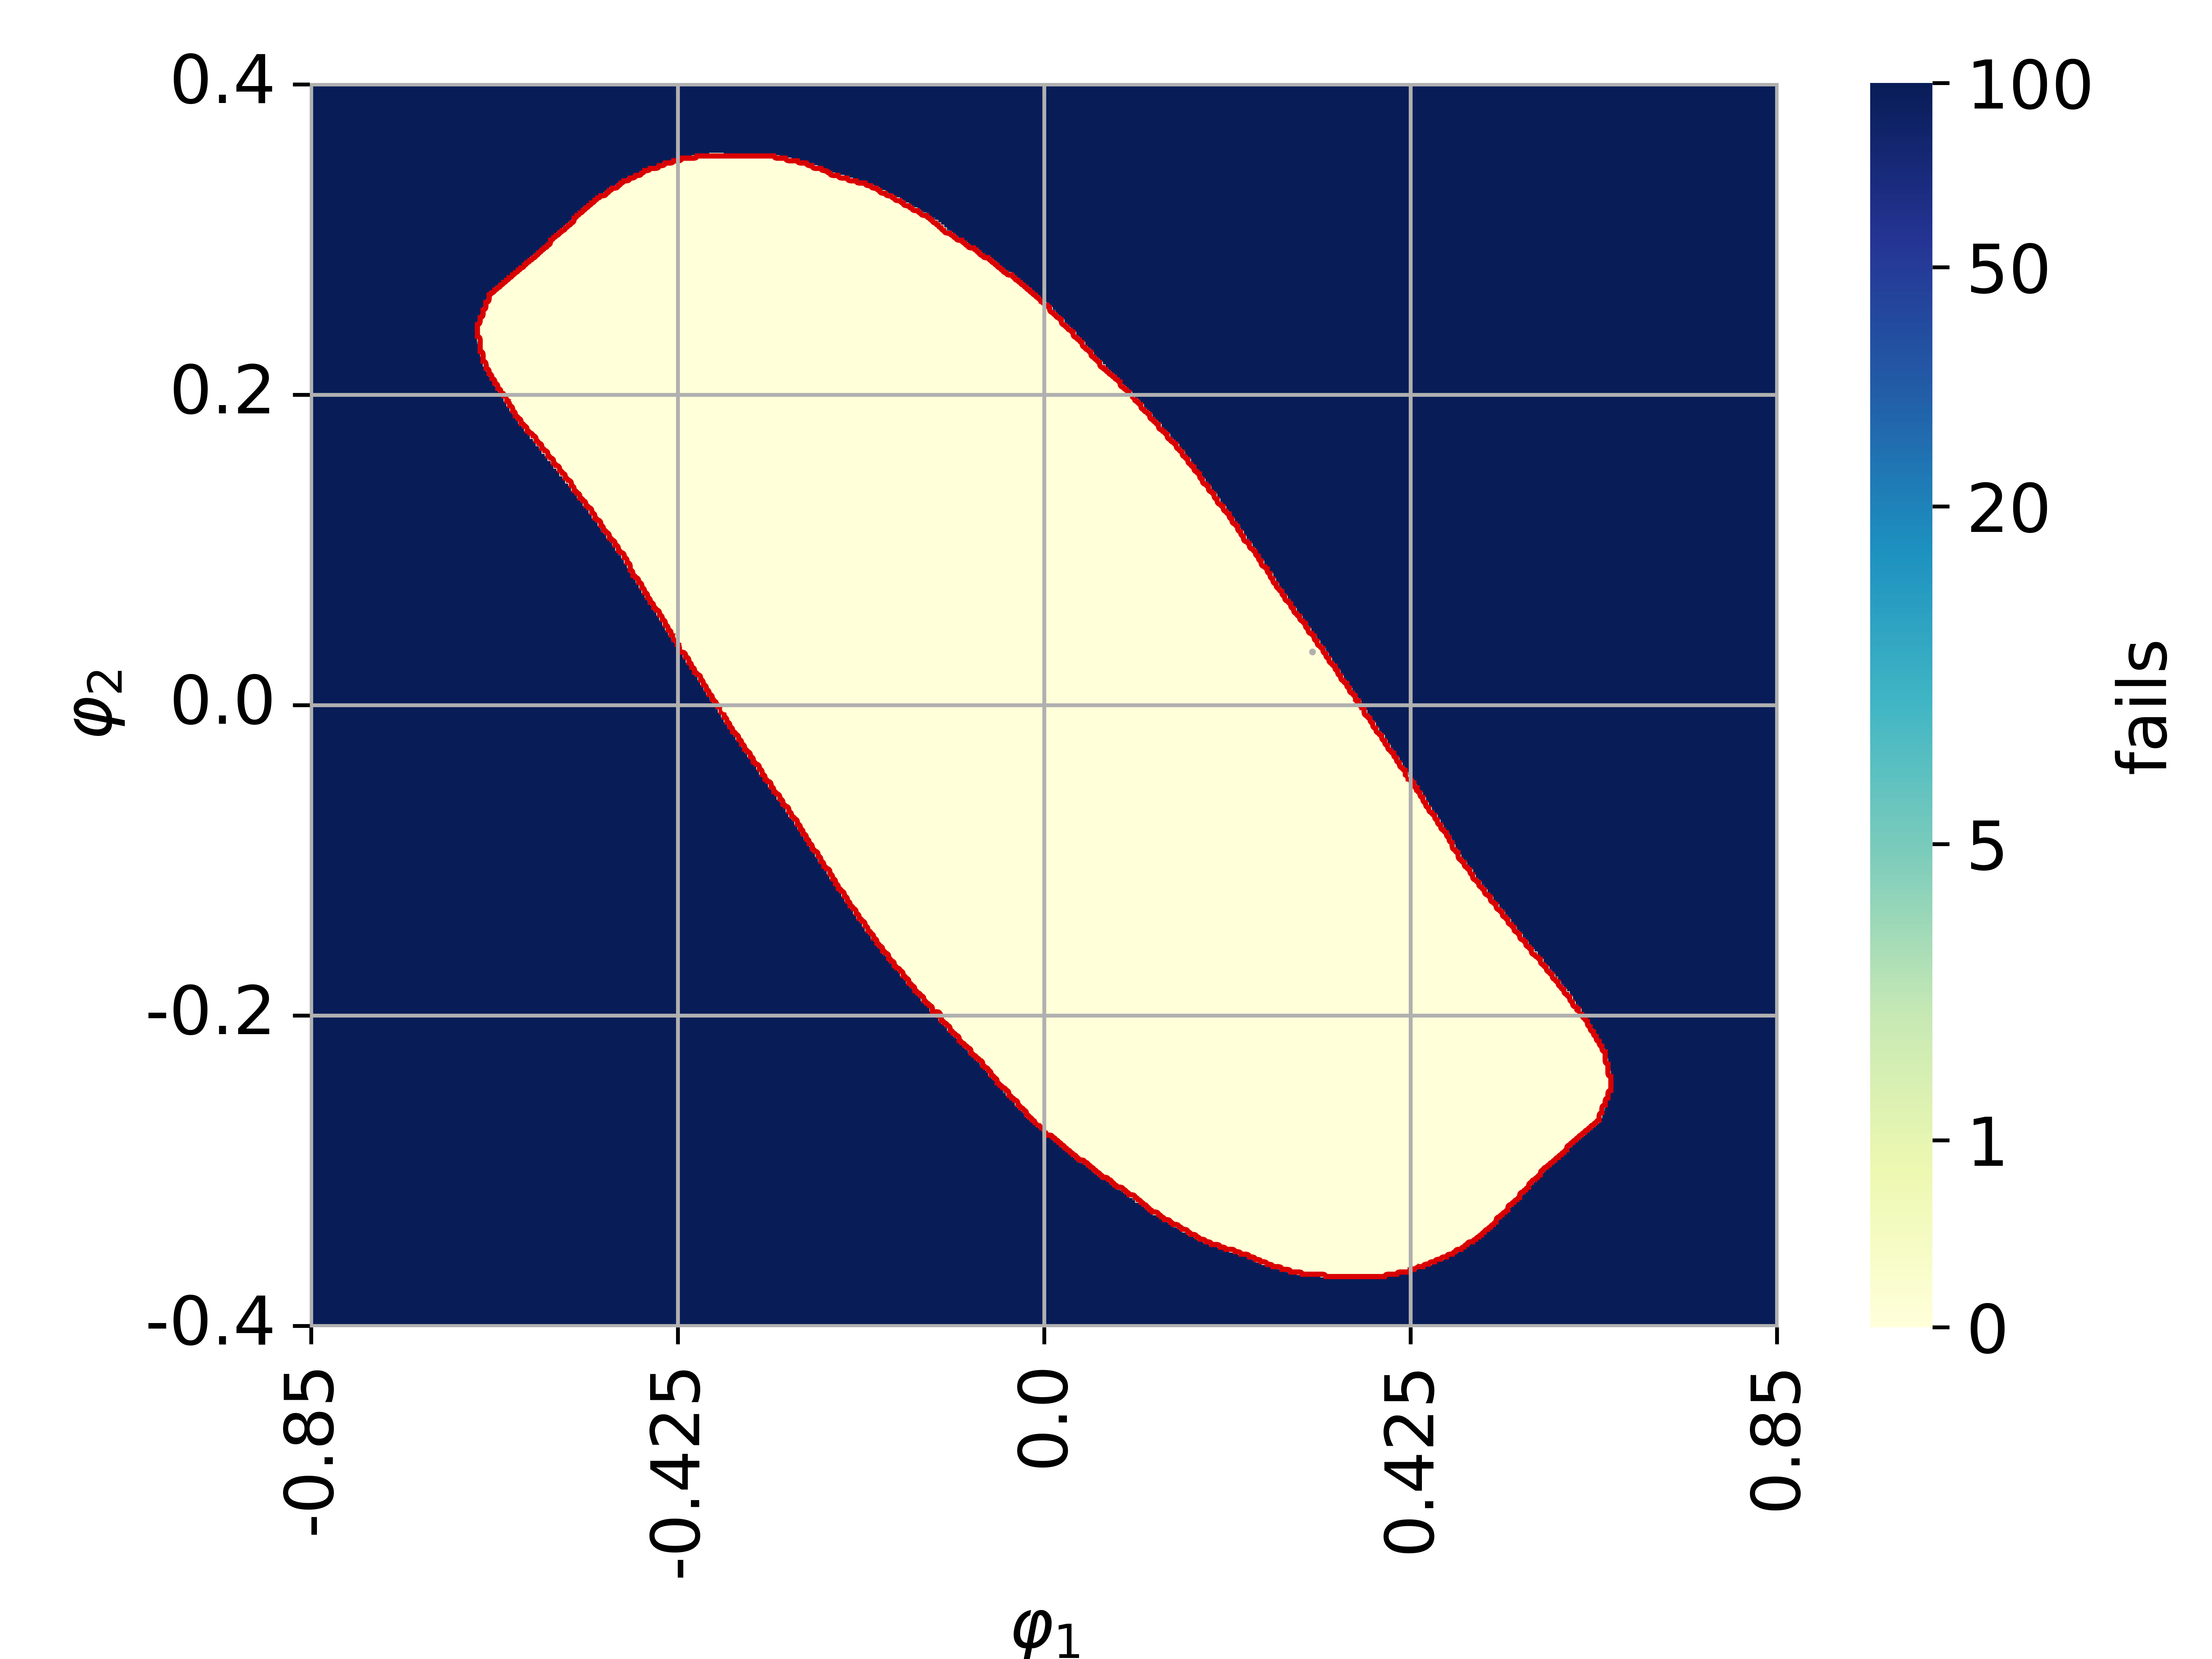
\includegraphics[width=\textwidth]{Figures/DP_mass_1.2.png}
         \label{fig: DP mass 1.2}
         \caption{}
     \end{subfigure}
     \hfill
     \begin{subfigure}[t]{0.32\textwidth}
         \centering
         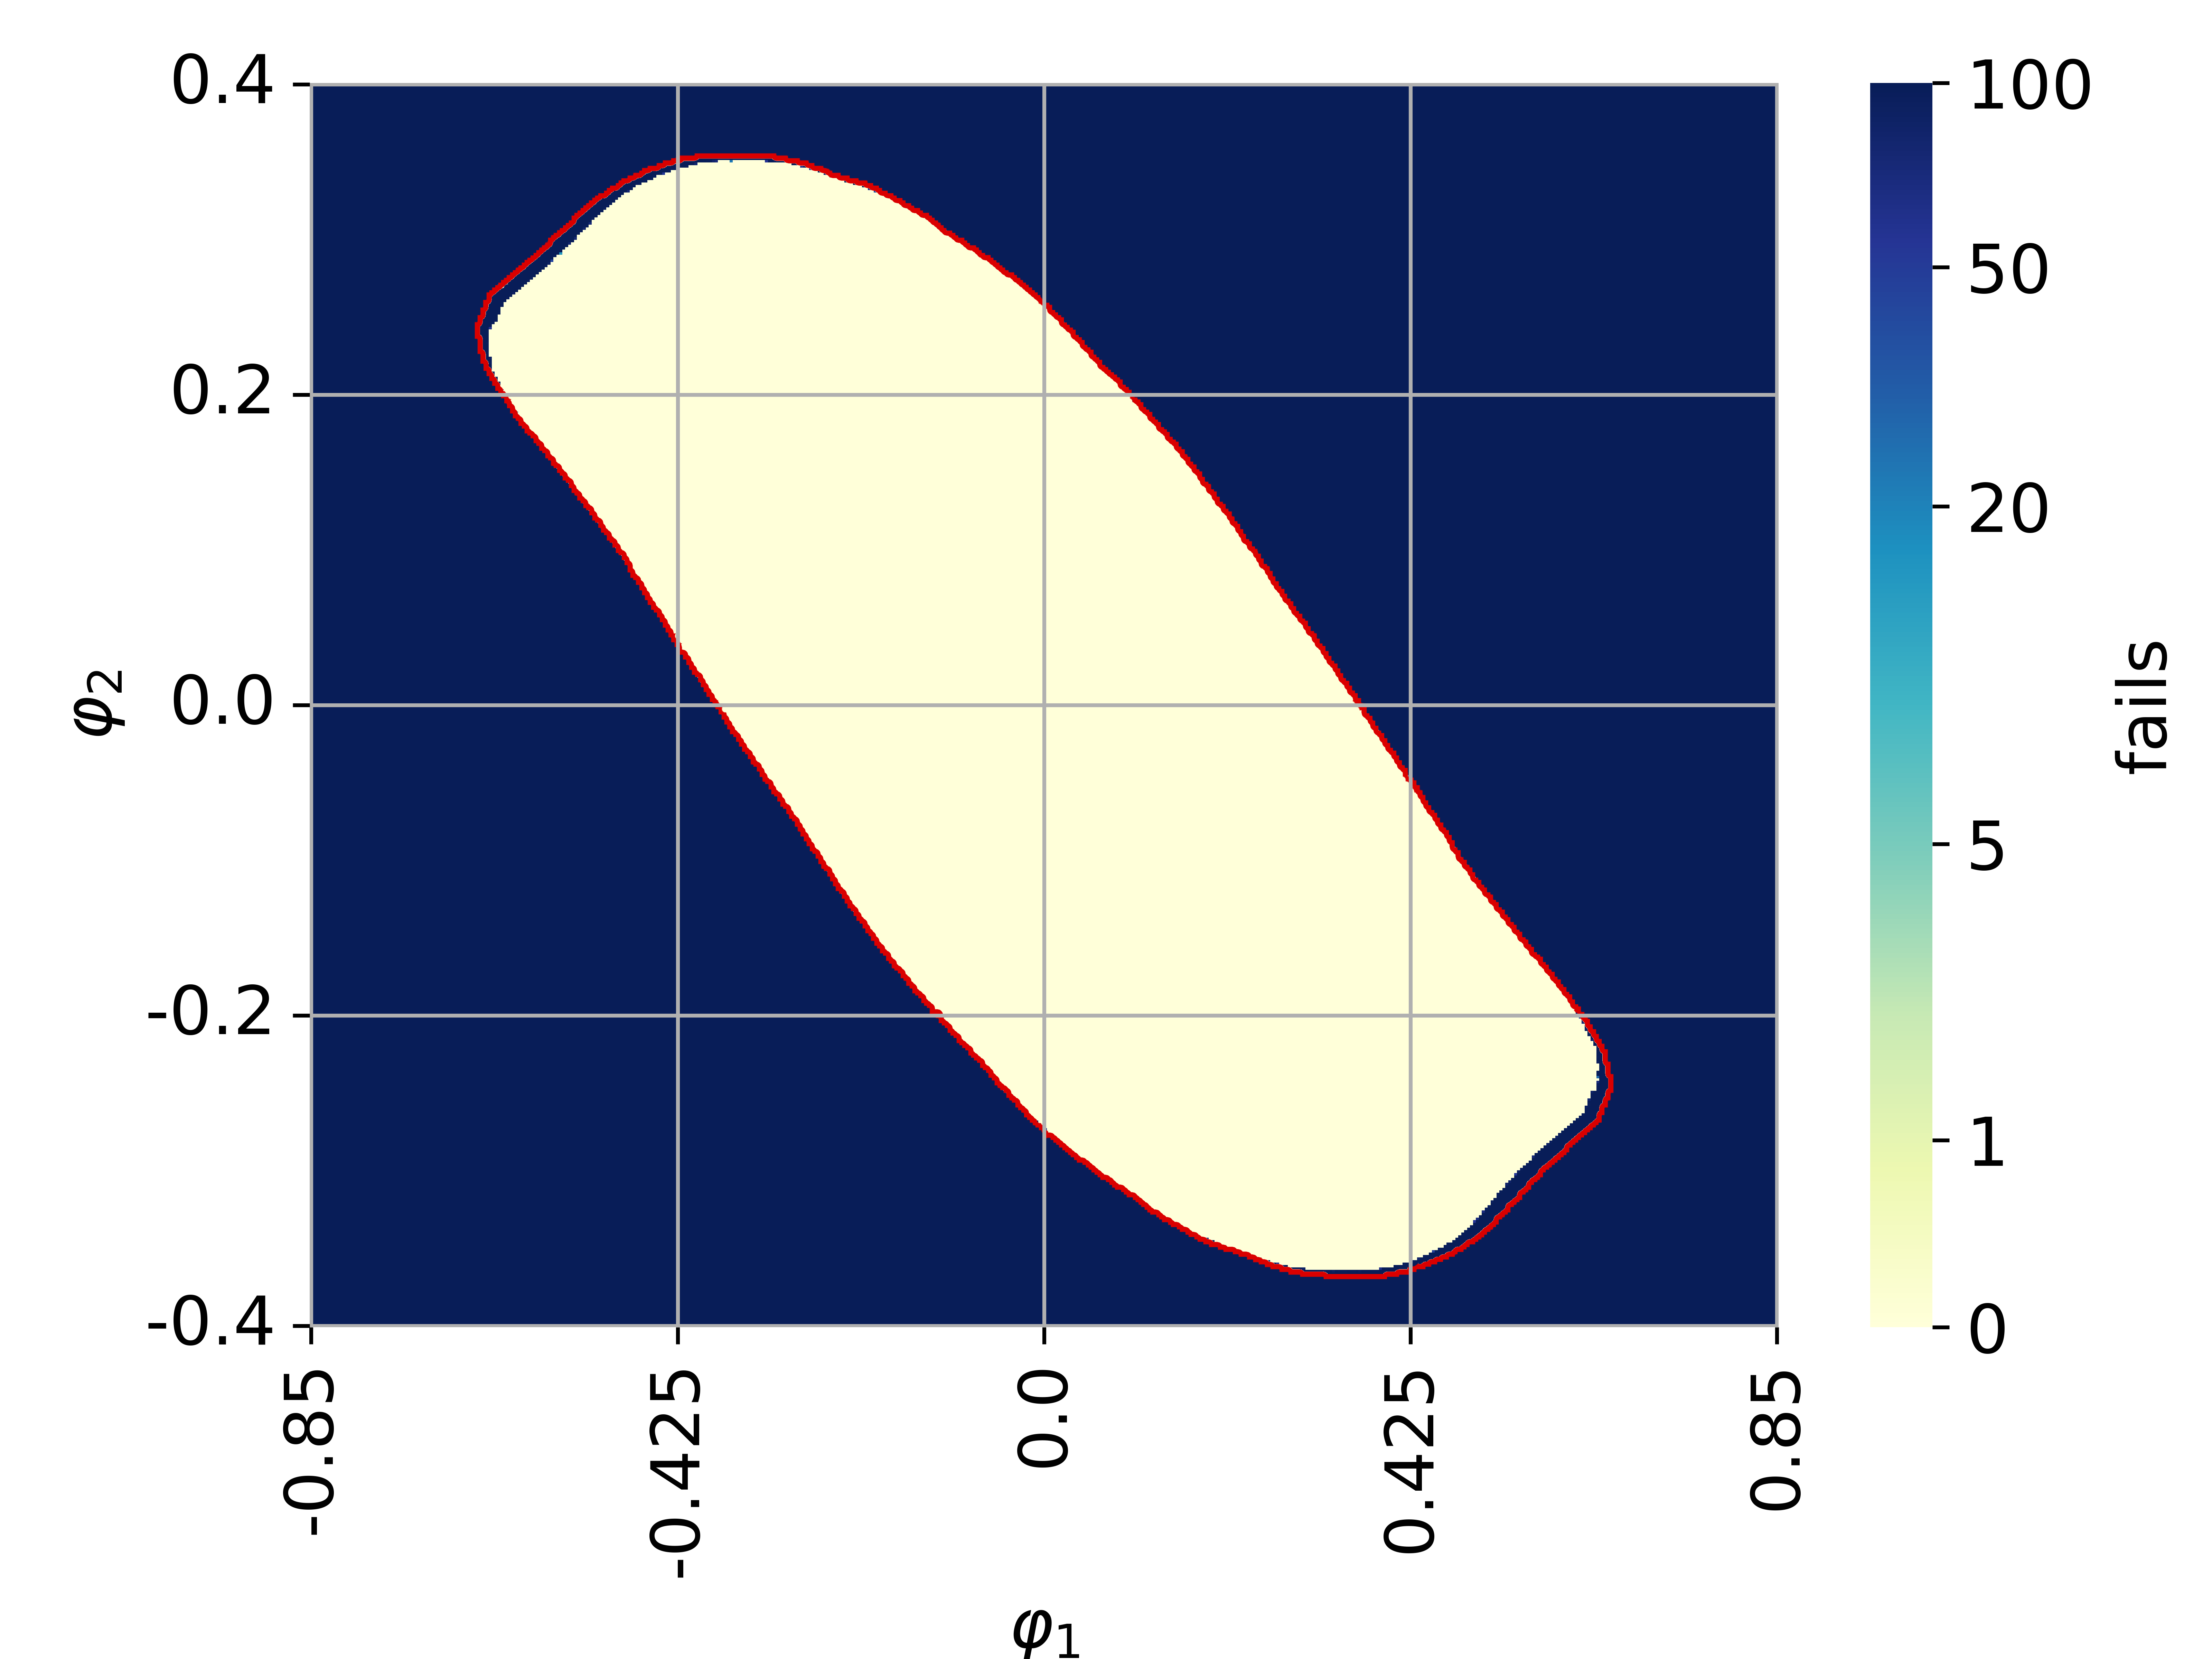
\includegraphics[width=\textwidth]{Figures/DP_friction_0.01.png}
         \label{fig: DP friction 0.01}
         \caption{}
     \end{subfigure}
     \hfill
     \begin{subfigure}[t]{0.32\textwidth}
         \centering
         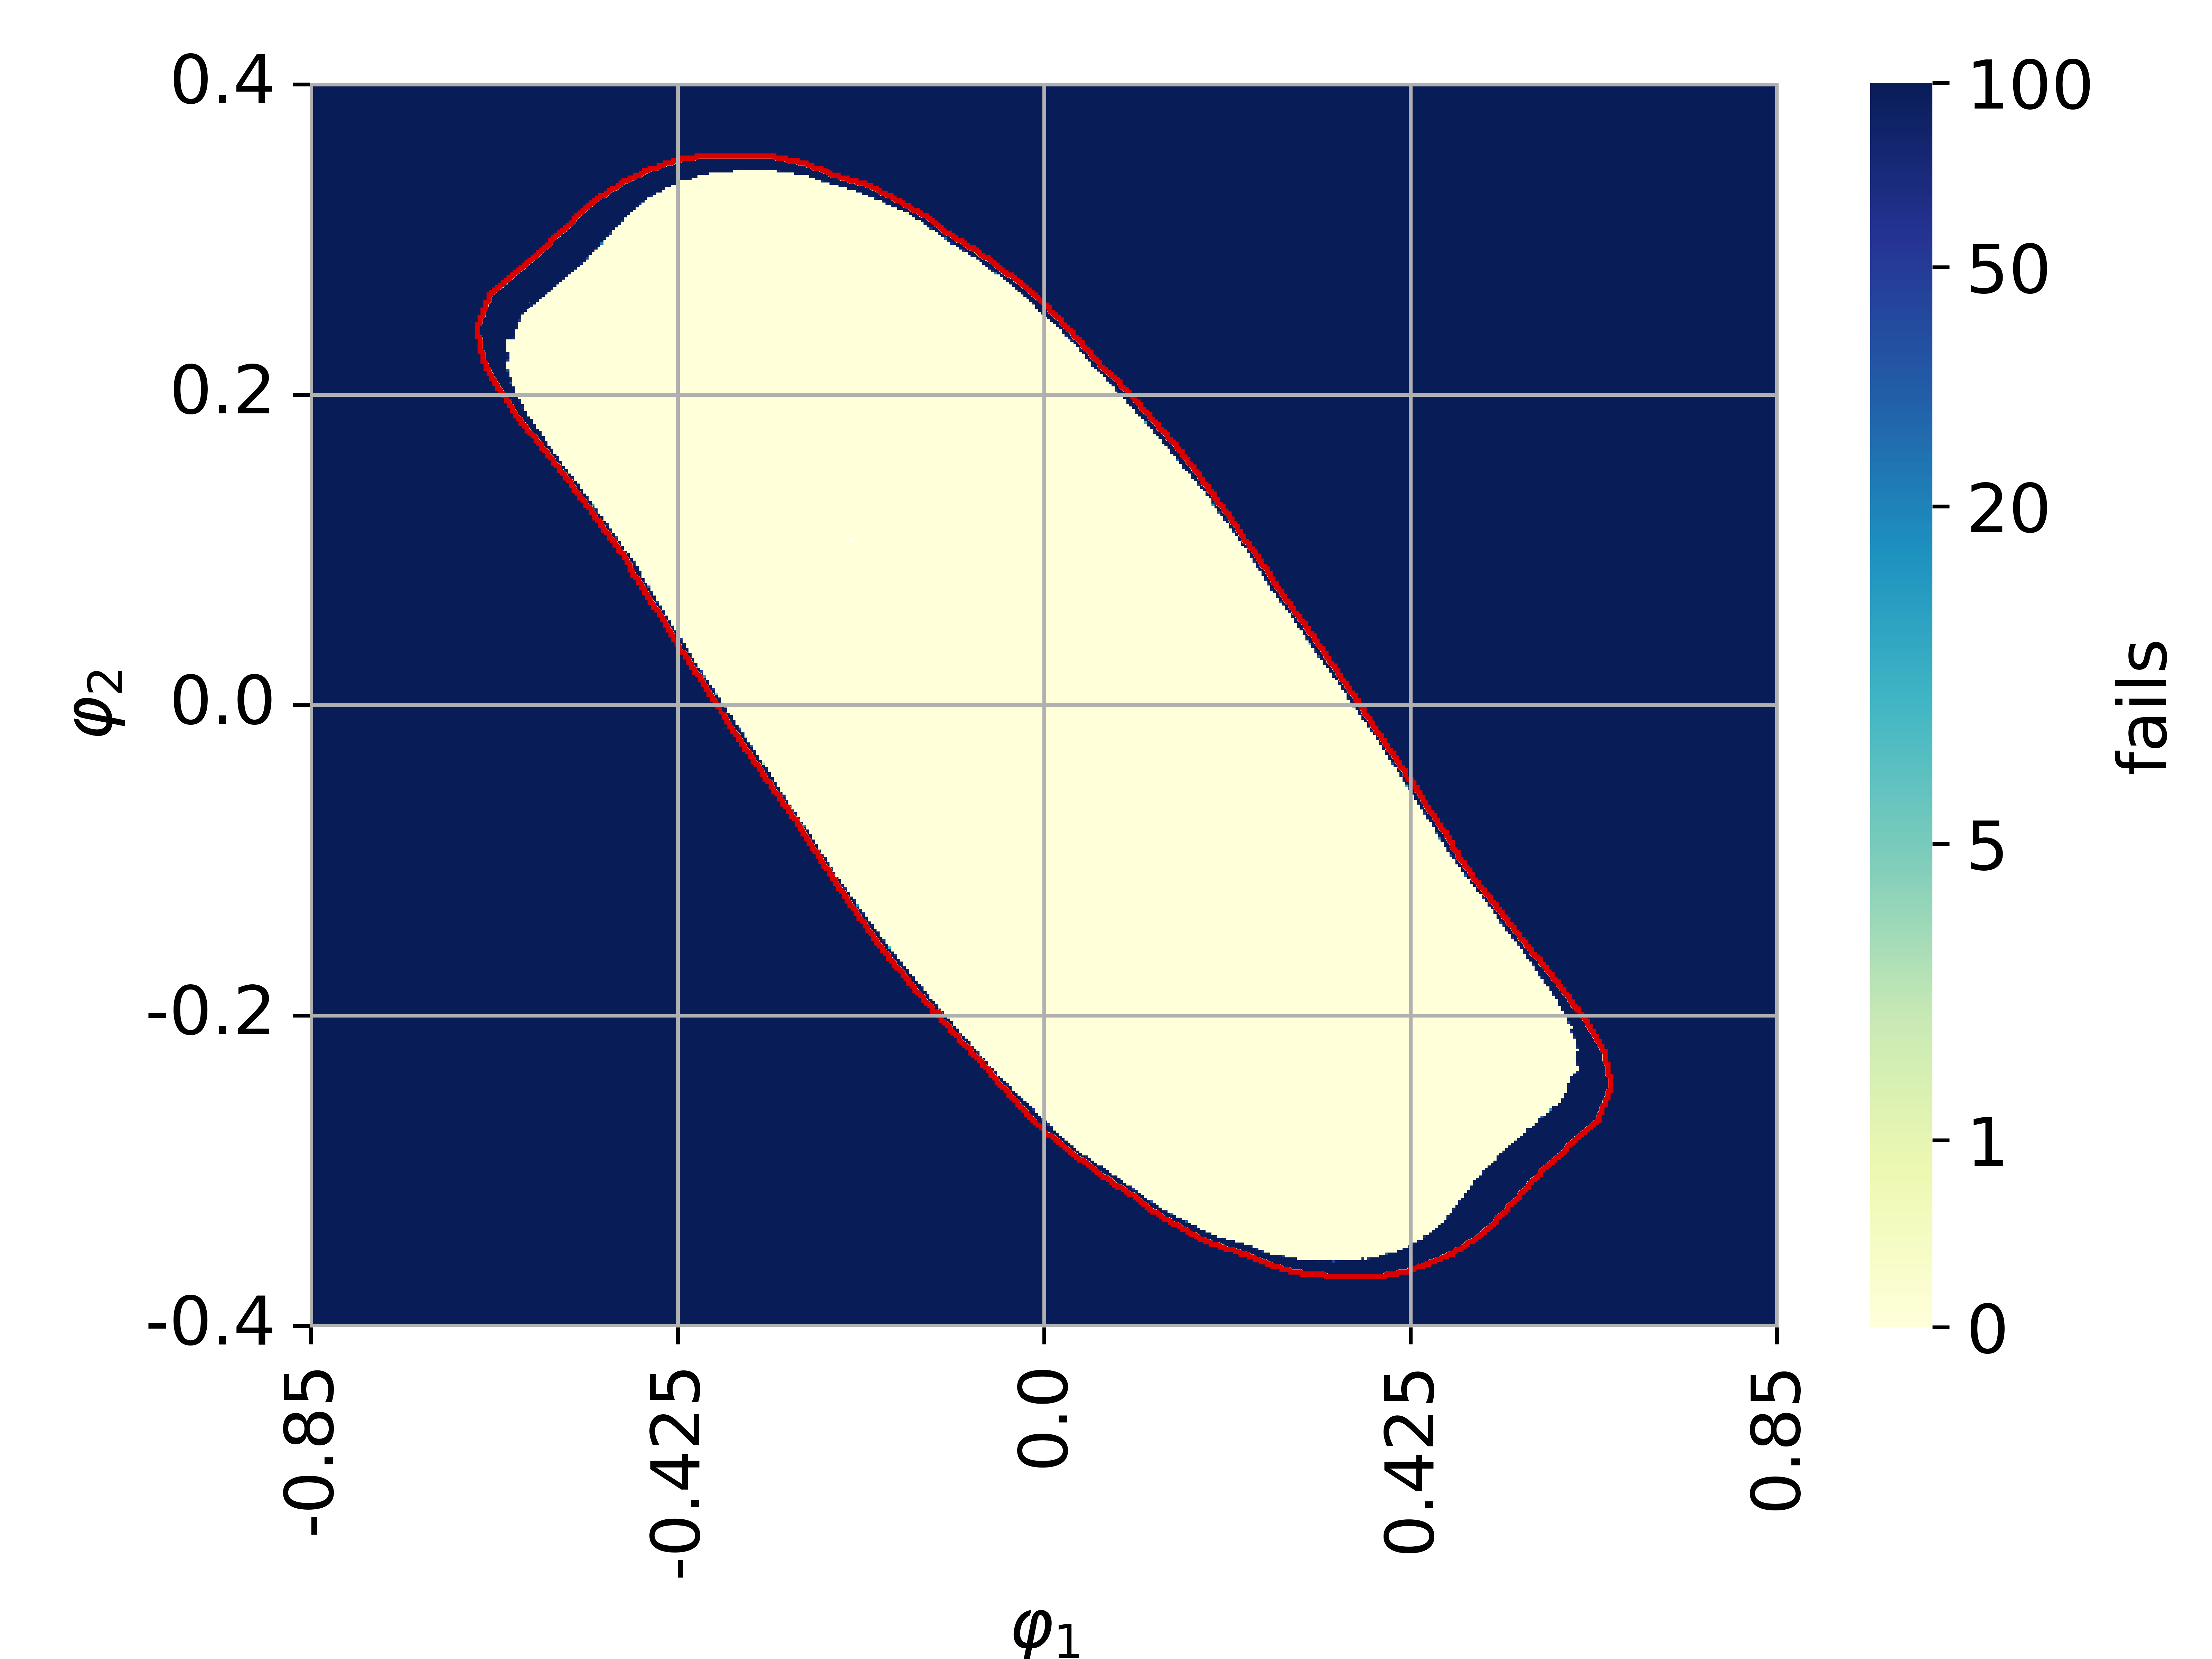
\includegraphics[width=\textwidth]{Figures/DP_friction_0.02.png}
         \label{fig: DP friction 0.02}
         \caption{}
     \end{subfigure}

     \caption{The stability zone for the double link system using the PPO agent, case 0. The red boundary corresponds to that depicted continuous control stability zone in Figure~\ref{fig: continuous vs discrete} (b). The environment parameters are modified as follows: (a) 1.1~$l$, (b) 1.2~$l$, (c) 1.1~$m$, (d) 1.2~$m$, (e) $f_{rel}$ = 0.01, and (f) $f_{rel}$ = 0.02.}
     \label{fig: agent impact on different environments}
 \end{figure}

The observations shows, that increasing the link length will cause the stability zone to expand (see Figures~\ref{fig: agent impact on different environments} (a) and (b)), while not having the increase of the blind spots, as it was for the discrete control cases~\cite{manzl2023relrl}. Increasing the mass of the link doesn't provide any differences from the base model (Figures~\ref{fig: agent impact on different environments} (c) and (d)), so that we can state that up to the changes of 20\% the model is independent from the link mass change, showing the same behavior as for the discrete model, where the changing of mass was also neglectable on the stability zones.
Considering friction the stability zone becomes smaller within each increase of it, but the value of \( f_{\text{rel}} = 0.02 \) still provides us with the stable zone without causing the agent to fail in the original contour (Figures~\ref{fig: agent impact on different environments} (e) and (f)), as it was shown in~\cite{manzl2023relrl}. It can be concluded that the continuous control scheme is more suitable if friction is involved in the environment model simulation.

\subsection{RL training enhancement with CL} \label{subsec: RL training enhancement with CL}

\textit{a) setting up a baseline}

Before proceeding with the analysis, it is essential to establish baseline results for the continuous RL PPO method, without enhancements from Curriculum Learning. This provides a point of reference to assess how much CL can improve performance. For this we have conducted tests using the system parameters presented in the Table~\ref{tab:hyperparameters} and~\ref{tab:env_params} for systems with 1 to 3 links. For each system, 10 distinct simulation cases were executed to account for variability in control due to different initial conditions. The baseline is determined by measuring the training timesteps required for success, focusing primarily on the mean and median values, which serve as the key performance indicators. Additionally, the minimum and maximum values provide insight into the range of results across cases. These metrics allow us to assess the general performance of PPO in continuous action space. Table~\ref{tab: baseline statistics for PPO in continuous action space} summarizes the results for the RL training using the PPO algorithm in continuous action space. The results are presented for systems with 1, 2, and 3 links.

\begin{table}[ht]
	\centering
	\caption{Baseline results of using PPO algorithm in continuous action space for 1 to 3 link pendulum systems}
	\begin{tabular}{@{}lccccc@{}}
		\toprule
		\textbf{System} & \textbf{Successful cases} & \textbf{Mean} & \textbf{Median} & \textbf{Minimum} & \textbf{Maximum} \\ \midrule
		\textit{1-link} & 10 & 26168 & 25600 & 24320 & 32000 \\
		\textit{2-link} & 7 & 48055 & 49152 & 38400 & 55296 \\
		\textit{3-link} & 5 & 278937 & 288768 & 194560 & 319488 \\ \bottomrule
	\end{tabular}
	\label{tab: baseline statistics for PPO in continuous action space}
\end{table}

As indicated in Table~\ref{tab: baseline statistics for PPO in continuous action space}, the results show a clear progression in training time as the system complexity increases from 1-link to 3-link. The 1-link system requires the least number of timesteps on average to reach successful training, while the 3-link system exhibits significantly higher values, with a mean training time nearly 10 times longer than the 1-link system. This demonstrates that as the system complexity increases, the training duration grows substantially, making it harder for the PPO algorithm to converge quickly.
The primary goal of introducing CL enhancement is to accelerate the training process and potentially make the system more robust to various initial conditions. By progressively increasing the difficulty of the tasks during training, we aim to reduce the number of timesteps required for convergence. To further explore the impact of CL, the next step focuses on selecting the appropriate CL implementation parameters, dividing the research into well-defined steps.

\textit{b) selection of a decay type (function)} 

At first, we shall determine which decay type is specifically the most performing for our particular task of pendulum stabilization. For this we have tested all described decay functions in subsection~\ref{subsec: Curriculum learning implementation} on a single pendulum system. With 150 runs per decay function of 5 initialization cases we use control values matrix of the form 
\(\begin{bmatrix} 1 & n \\ 0 & 0 \end{bmatrix}\), where \(n = 2, 4, 6, 8, 10\) and decay steps vector \(\begin{bmatrix} 0 \\ k \end{bmatrix}\), where \(k = 5000, 6000, \ldots, 10000\) to evaluate the performance across different control parameters. The results are presented in a form of a bar plot, which shows the number of agent successes for the whole dataset (see Figure~\ref{fig: decay types comparison}).  

\begin{figure}[h]
	\centering
	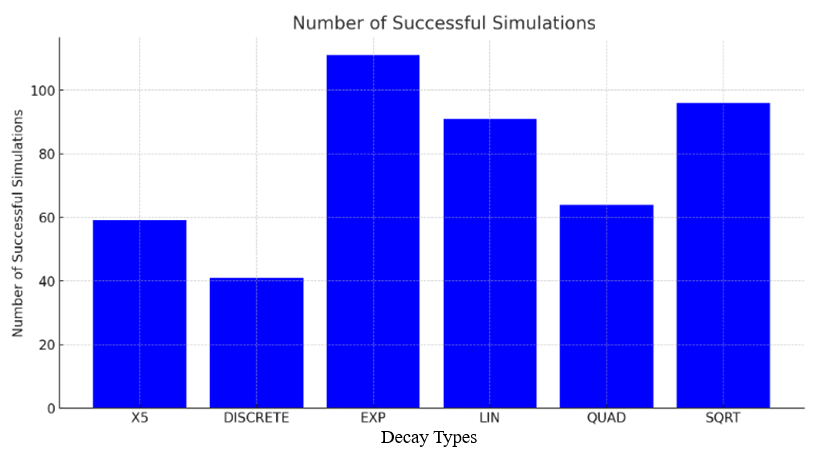
\includegraphics[width=12cm]{Figures/decay_types_results_comparison.png}
	\caption{Simulation results for decay types analysis. Each bar plot represents the value of successfully trained cases out of 150 in total per decay function.}
	\label{fig: decay types comparison}
\end{figure}

The exponential decay function, provides the best results of having 74\% of successes across the dataset and therefore will be considered as the main function used in our next analysis. 

\textit{c) selection of decay factor}

For the selection of the decay factor, we performed an extensive analysis using a double pendulum system. The control values matrix was set as \(\begin{bmatrix} 1 & n & n \\ 0 & 0 & 0 \end{bmatrix}\), where \(n = 1, 2, \ldots, 10\). The decay steps, which represent how long the curriculum learning is conducted, were varied from 9000 to 22000 with increments of 1000. For each unique combination of control values, decay steps, and decay factors, we executed 10 cases to ensure the reliability and robustness of our results. In total, we analyzed 4 decay factors: 0.005, 0.01, 0.05, and 0.5, generating a dataset with approximately 70,000 lines of results. The objective of this analysis was to determine the optimal decay factor for maximizing the system's learning performance.
The output metric used for comparison included the value of training timesteps. This metric provide insight into how efficiently the system is able to solve tasks within the corresponding timesteps.

\begin{figure}[h] 
	\centering 
	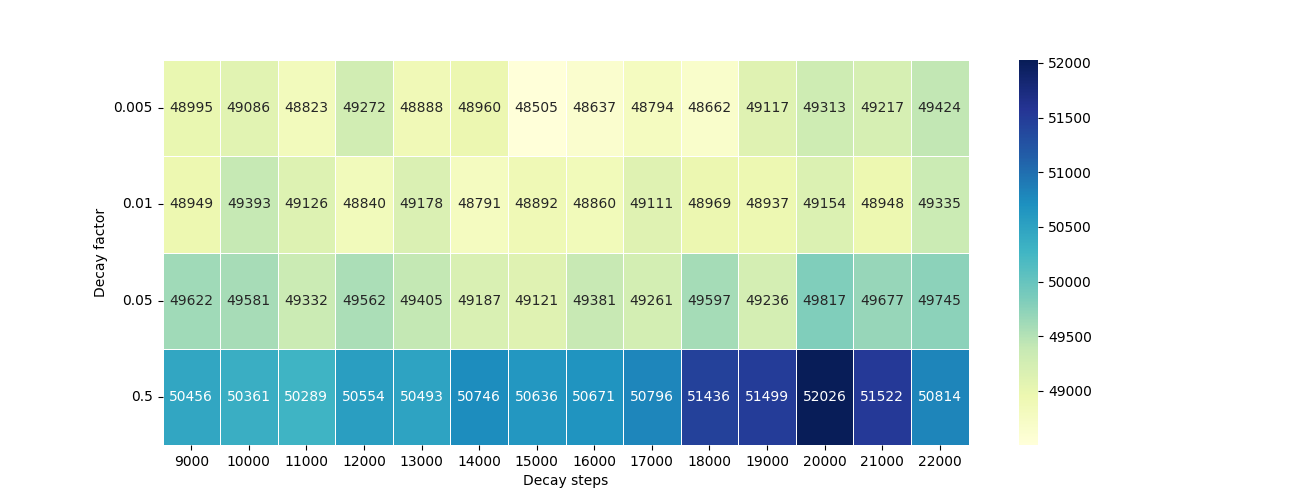
\includegraphics[width=15cm]{Figures/MaxSuccessfulTestsTimesteps_heatmap.png} 
	\caption{Heatmap showing the impact of different decay factors on the number of successful tests and timesteps. The decay factor 0.005 consistently performs best in terms of minimizing timesteps.} 
	\label{fig: decay factors comparison}
\end{figure}

As shown in Figure~\ref{fig: decay factors comparison} decay factor 0.005 consistently results in the lowest timesteps across all combinations of control values and decay steps. This indicates that the system converges faster and more efficiently with a decay factor of 0.005 compared to the other decay factors. The smaller the timesteps, the faster the system is able to learn, making 0.005 the most optimal choice for our training setup.

\textit{d) applying CL enhancement}

The next step in our analysis involves the development of a control value decay scheme to assess its influence while varying decay steps. For the single pendulum system, the control values matrix is maintained as \(\begin{bmatrix} 1 & n \\ 0 & 0 \end{bmatrix}\), since the simplicity of the system allows for efficient training without requiring significant constraints on movement. Experiments were conducted by varying $n$ from 0.1 to 1 (step size of 0.1), and from 1 to 12 (step size of 1). Decay steps ranged from 1000 to 12000, with increments of 1000. 
For the double pendulum system, the control scheme was set as \(\begin{bmatrix} 1 & c \cdot n & r \cdot n \\ 0 & 0 & 0 \end{bmatrix}\), where $c$ and $r$ represent extension coefficients used to observe the effects of pendulum link constraint magnitudes on the results and are varied over the set \({1, 2, 4, 8}\), while \(n = 1, 2, \ldots, 10\). Decay steps were varied between 9000 and 22000, with an increment of 1000. 
For the triple link system, the control scheme used was \(\begin{bmatrix} 1 & 4n & 2n & n \\ 0 & 0 & 0 & 0 \end{bmatrix}\), where \(n = 1, 2, \ldots, 10\). This configuration required stronger restrictions on the first link due to its responsibility in bearing the mass of the subsequent links. The decay steps were varied between 30000 and 50000, with increments of 1000.
The evaluation of results was performed across cases within each unique combination of control values and decay steps, rather than across the entire control scheme. This is due to the CL implementation, which focuses on enhancing training efficiency where the key factor is to find the optimal combination of values to facilitate faster and more robust learning in the system. To determine the best-performing combination of control values and decay steps, we concentrated on three primary factors: number of successful cases in each combination, mean and median values of training time across cases. For the single and double pendulum systems, a successful case was defined as achieving 50 out of 50 successful tests. For the triple pendulum system, due to its higher complexity, the threshold for success was set at 70 out of 100 tests passed. This adjustment reflects the increased difficulty of achieving full success for the triple link system. The results are shown in the Table~\ref{tab: CL results}.

\begin{table}[ht]
	\centering
	\caption{CL enhancement: best results for 1 to 3 link pendulum systems}
	\begin{tabular}{@{}lccccc@{}}
		\toprule
		\textbf{System} & \makecell{\textbf{Best performing}\\ \textbf{schemes}} & \makecell{\textbf{Successful}\\ \textbf{cases}} & \makecell{\textbf{Decay}\\ \textbf{steps}} & \textbf{Mean} & \textbf{Median} \\ \midrule
		\textit{1-link} & \(\begin{bmatrix} 1 & 0.8 \\ 0 & 0 \end{bmatrix}\) & 10 & 7000 & 17817 & 18432 \\ \midrule
		\textit{2-link} & \(\begin{bmatrix} 1 & 20 & 5 \\ 0 & 0 & 0 \end{bmatrix}\) & 10 & 15000 & 43929 & 43008 \\ \midrule
		\textit{3-link} & \(\begin{bmatrix} 1 & 16 & 8 & 4 \\ 0 & 0 & 0 & 0 \end{bmatrix}\) & 10 & 30000 & 233676 & 216064 \\ \bottomrule
	\end{tabular}
	\label{tab: CL results}
\end{table}

The results in Table~\ref{tab: CL results} demonstrate the effectiveness of the best-performing control schemes across the three systems, with all systems achieving 10 out of 10 successful cases. These results highlight the robustness of the implemented Curriculum Learning in reducing training times while maintaining high success rates, even as system complexity increases.
To gain further insights into how the variations in control schemes and decay steps influenced the training times, we present a series of heatmaps showed on Figure~\ref{fig: percentage heatmaps for 1- to 3- link systems using CL} (a) to (f). The percentage change in both mean and median training times for each pendulum system is visualized, offering a clear depiction of the impact of CL enhancements across different cases.

\begin{figure}[h!]
	\centering
	\begin{subfigure}[t]{0.32\textwidth}
		\centering
		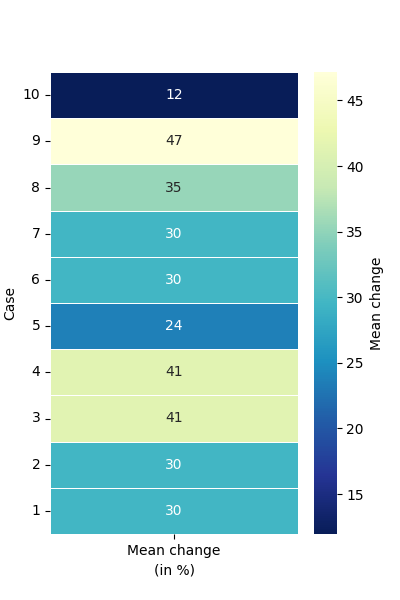
\includegraphics[width=\textwidth]{Figures/SP_mean_heatmap_percentage.png}
		\label{fig: SP_mean}
		\caption{}
	\end{subfigure}
	\hfill
	\begin{subfigure}[t]{0.32\textwidth}
		\centering
		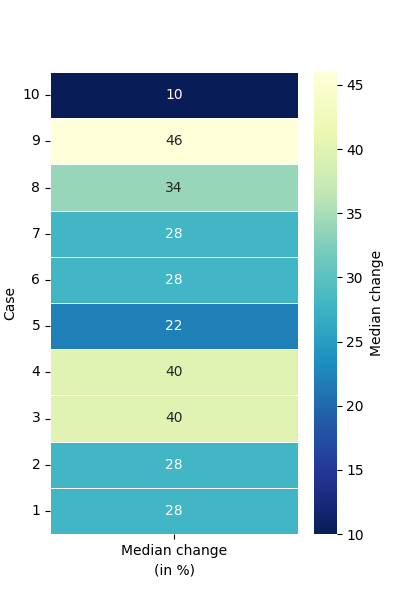
\includegraphics[width=\textwidth]{Figures/SP_median_heatmap_percentage.png}
		\label{fig: SP_median}
		\caption{}
	\end{subfigure}
	\hfill
	\begin{subfigure}[t]{0.32\textwidth}
		\centering
		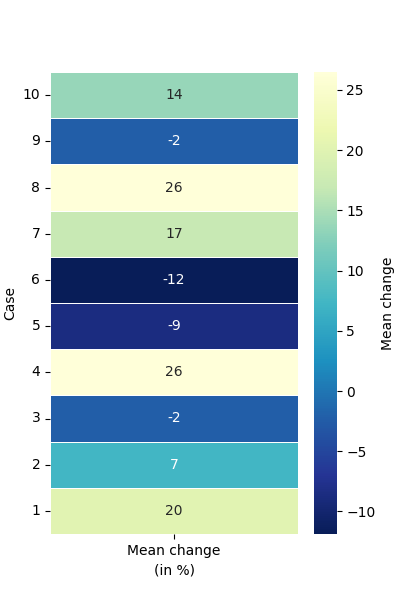
\includegraphics[width=\textwidth]{Figures/DP_mean_heatmap_percentage.png}
		\label{fig: DP_mean}
		\caption{}
	\end{subfigure}
	
	\vspace{0.2cm}
	
	\begin{subfigure}[t]{0.32\textwidth}
		\centering
		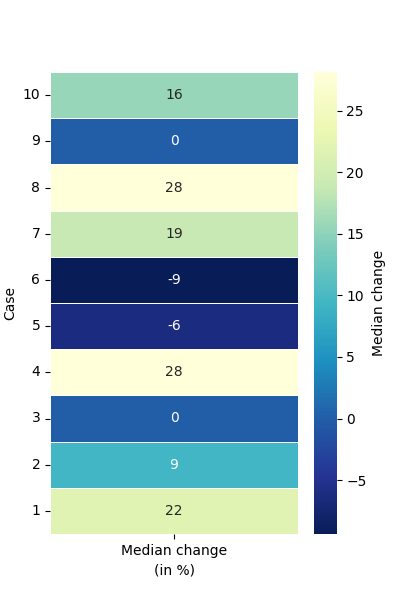
\includegraphics[width=\textwidth]{Figures/DP_median_heatmap_percentage.png}
		\label{fig: DP_median}
		\caption{}
	\end{subfigure}
	\hfill
	\begin{subfigure}[t]{0.32\textwidth}
		\centering
		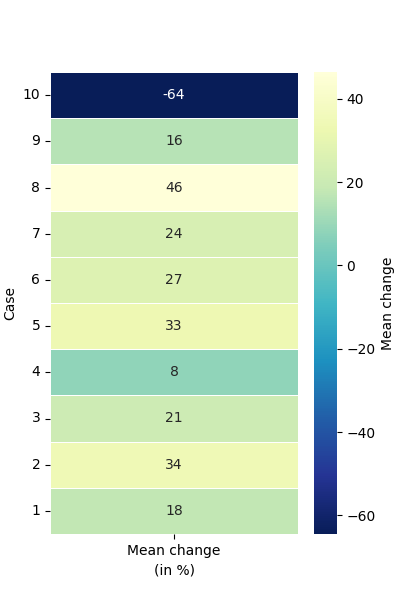
\includegraphics[width=\textwidth]{Figures/TP_mean_heatmap_percentage.png}
		\label{fig: TP_mean}
		\caption{}
	\end{subfigure}
	\hfill
	\begin{subfigure}[t]{0.32\textwidth}
		\centering
		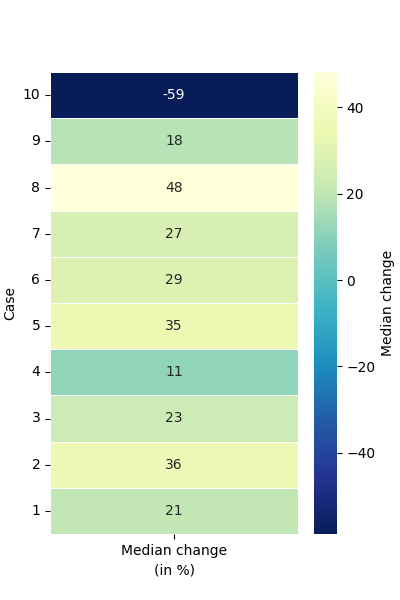
\includegraphics[width=\textwidth]{Figures/TP_median_heatmap_percentage.png}
		\label{fig: TP_median}
		\caption{}
	\end{subfigure}
	
	\caption{Mean and median training time change per cases for 1- to 3- link pendulum systems using CL enhancement.}
	\label{fig: percentage heatmaps for 1- to 3- link systems using CL}
\end{figure}

The heatmaps clearly demonstrate that, across all systems, the implementation of CL resulted in a substantial improvement in training speed. The 1-link system showed the greatest consistency, while the 2-link and 3-link systems demonstrated significant improvements in reduced training time.

\begin{table}[ht]
	\centering
	\caption{Improvement statistics by enhancing RL training of the 1 to 3 link pendulum systems with CL}
	\begin{tabular}{@{}lcc@{}}
		\toprule
		\textbf{System} & \makecell{\textbf{Mean}\\ \textbf{improvement}} & \makecell{\textbf{Median}\\ \textbf{improvement}} \\ \midrule
		\textit{1-link} & 32\% & 28\% \\
		\textit{2-link} & 8.6\% & 12.5\% \\
		\textit{3-link} & 19\% & 25.2\% \\ \bottomrule
	\end{tabular}
	\label{tab: CL improvement statistics}
\end{table}

The results in Table~\ref{tab: CL improvement statistics} indicate that the Curriculum Learning (CL) enhancement has proven effective in reducing training times and improving the robustness of reinforcement learning across all systems. While the 1-link system showed the greatest improvement, with a 32\% reduction in mean training time, the double and triple pendulum systems also exhibited substantial improvements, confirming the scalability of CL to more complex multi-link systems. This success demonstrates that CL enables the RL agent to better navigate the increased complexity of the tasks, allowing it to converge more efficiently. 
One of the most important findings is that all systems, including the 2-link and 3-link systems, reached 10 out of 10 successful cases. This confirms that the control schemes used, combined with CL, were able to handle even the more complex tasks. By gradually increasing the difficulty of the tasks during training, CL helps the reinforcement learning agent learn more effectively, avoiding large jumps in difficulty that could slow down training or cause failure. The heatmaps provided earlier also showed consistent improvement in training time across different control values and decay steps, meaning that the benefits of CL are not limited to specific parameters. This makes CL a powerful and flexible tool for improving reinforcement learning across a wide range of scenarios. However, it’s important to recognize that finding the best parameters (such as control values and decay steps) is still key to maximizing the benefits of CL. While our results show significant improvements, further fine-tuning could make the training even faster, especially in more complicated systems. Future research could focus on dynamic approaches where the curriculum adjusts based on the agent's performance during training, potentially leading to even better results.
In summary, Curriculum Learning has proven to be an effective way to speed up training and improve robustness in all systems tested. From the simpler 1-link pendulum to the more challenging 3-link system, CL has provided consistent improvements, making it a valuable strategy in reinforcement learning. These findings show the importance of a well-planned training process and suggest future possibilities for even greater gains with more advanced strategies.